\documentclass[10pt,journal,compsoc]{IEEEtran}

\usepackage{cite}
\usepackage{amsmath,amssymb,amsfonts}
\usepackage{algorithmic}
\usepackage{graphicx}
\usepackage{textcomp}
\usepackage{xcolor}
\usepackage{booktabs}
\usepackage{url}
\usepackage[hidelinks]{hyperref}
\renewcommand{\thetable}{\Roman{table}}
\def\BibTeX{{\rm B\kern-.05em{\sc i\kern-.025em b}\kern-.08em
    T\kern-.1667em\lower.7ex\hbox{E}\kern-.1252emX}}

\setlength{\textfloatsep}{5pt plus 1pt minus 1pt}
\setlength{\floatsep}{4pt plus 1pt minus 1pt}
\setlength{\intextsep}{4pt plus 1pt minus 1pt}
\setlength{\dbltextfloatsep}{5pt plus 1pt minus 1pt}
\setlength{\dblfloatsep}{4pt plus 1pt minus 1pt}
\setlength{\abovecaptionskip}{3pt plus 1pt minus 1pt}
\setlength{\belowcaptionskip}{3pt plus 1pt minus 1pt}

\begin{document}
\title{Stress-Testing Preference Elicitation in Instruction-Tuned Language Models: Separating Commitment, Conditional Direction, and Payoff Sensitivity Across Small Model Families}

\author{Shriyam Baloni, Achin Jain, Debojyoti Roy, Vanita Jain, and Massimo Donelli%
\IEEEcompsocitemizethanks{\IEEEcompsocthanksitem S. Baloni, A. Jain, and D. Roy are with the Department of Computer Engineering, University of Delhi, Delhi 110007, India (e-mail: karanbaloni@ce.du.ac.in; achin.mails@gmail.com; roydebojyoti16@gmail.com).%
\IEEEcompsocthanksitem V. Jain is with the Department of Electronics and Communication Engineering, Faculty of Technology, University of Delhi, Delhi 110007, India (e-mail: vanitajain@fot.du.ac.in).%
\IEEEcompsocthanksitem M. Donelli is with the Department of Information Engineering and Computer Science, University of Trento, 38123 Trento, Italy (e-mail: massimo.donelli@unitn.it).}%
\thanks{Manuscript received November 2026. Corresponding author: Achin Jain (e-mail: achin.mails@gmail.com).}}

\IEEEtitleabstractindextext{%
\begin{abstract}Standard language-model preference evaluations use forced-choice protocols compelling models to choose between directional actions, conflating whether an agent commits to action with which option it selects. We propose a behavioral diagnostic separating directional commitment from conditional payoff sensitivity via an explicit \textit{Indifferent} option. Across 4,480 consequential trials across four small model families (Qwen 2.5 3B, Llama 3.2 3B, Phi-4 Mini 3.8B, Gemma 3 4B) and 20 decision dilemmas, forced choice obscures fundamental behavioral divergences. When permitted to decline directional action, directive models (Llama, Phi, Gemma) commit in $\ge 96\%$ of trials, whereas Qwen 2.5 3B abstains on 85.3\% of trials. Conditional on committing, Qwen displays apparent payoff sensitivity ($\hat\beta = 1.231$, 95\% CI [0.50, 1.96]$ under Firth regression) that is heavily position-moderated under default labels (dropping to 49.0\% in the disfavored slot), though neutral counterbalancing eliminates this asymmetry. Llama and Phi exhibit moderate sensitivity ($\hat\beta = 0.282$ and $0.225$), while Gemma shows near-ceiling sensitivity ($\hat\beta = 1.531$). Counterbalancing reveals that Qwen's abstention is moderated by action semantics (jumping from 16.8\% to 87.6\% disparity commitment across 1,120 trials). Furthermore, matched forced choice compels Qwen into an extreme 79:21 positional imbalance at parity, showing that forced choice can manufacture directional bias.
\end{abstract}

\begin{IEEEkeywords}
Large Language Models, AI Evaluation, Revealed Preferences, Behavioral Economics, Construct Validity
\end{IEEEkeywords}}

\maketitle
\markboth{IEEE Open Journal of the Computer Society}{Baloni \MakeLowercase{\textit{et al.}}: Stress-Testing Preference Elicitation in Instruction-Tuned Language Models}
\IEEEdisplaynontitleabstractindextext
\IEEEpeerreviewmaketitle

\section{Introduction}
\label{sec:introduction}

The deployment of Large Language Models (LLMs) as autonomous or semi-autonomous agents has accelerated efforts to characterize model behavior in terms of values, utility, preferences, and alignment with human objectives. A common strategy is to present a model with multiple alternatives and infer a directional preference from the selected option. Such protocols are attractive because they transform a complex behavioral question into a measurable output. Yet the mapping from an observed output to a latent construct is not automatic: a directional response can arise because the model has a robust preference, because the prompt induces a positional or linguistic bias, because the model is resolving an ambiguity, or because the protocol simply requires a choice even when the alternatives are not meaningfully distinguished.

This distinction creates a measurement problem for preference elicitation. In a conventional two-alternative forced-choice (2AFC) design, the model must select one of two alternatives. Consequently, the protocol cannot directly distinguish a directional commitment from a non-directional outcome that would have been expressed as indifference, abstention, or neutrality if such an option were available. Recent work has shown that elicitation protocol can materially affect the relationship between stated and behaviorally revealed choices, including when models are allowed to abstain \cite{mind_the_gap_2026}. While models can exhibit structured utility functions under standard forced-choice elicitation \cite{mazeika2025utility}, apparent alignment rankings and preference evaluations frequently show severe measurement instability under procedural variation \cite{randomness_not_rep_2025}. Separate evidence also shows that language-model choices can depend sensitively on presentation order, framing, and response formatting \cite{fragile_preferences_2026,innate_econ_preferences_2026,zheng2023large}. Taken together, these findings motivate an evaluation decomposition that asks not only \emph{which} option is selected, but also \emph{whether the model commits directionally at all}.

The present study develops and evaluates such a decomposition in a consequential, multi-turn task environment. The task provides the model with two operations, referred to as \textit{Add} and \textit{Subtract}, whose consequences are associated with quantitatively specified quality payoffs. An explicit \textit{Indifferent} response is always available alongside the directional options at the initial decision turn. The payoff ratio is manipulated parametrically from 1:9 through 9:1, allowing the study to distinguish signed preference direction from payoff-magnitude sensitivity. Presentation position is crossed independently with payoff dominance, yielding a balanced factorial design across 20 structural dilemmas. Selecting a directional action triggers a consequential downstream state update (Turn~2) and a follow-on decision (Turn~3), while selecting \textit{Indifferent} skips further processing. This embeds choice within an operational task pipeline rather than an abstract questionnaire.

We evaluate this protocol across four locally deployed (via Ollama; publicly released pre-trained model weights, not locally fine-tuned) instruction-tuned models in the 3--4B parameter class (Qwen 2.5 3B, Llama 3.2 3B, Phi-4 Mini 3.8B, and Gemma 3 4B) under deterministic greedy decoding ($T=0.0$). We find that allowing an explicit non-directional response reveals substantial cross-model heterogeneity that would be invisible in a standard forced-choice design. One model (Qwen 2.5) abstained in 85.3\% of valid trials, reserving directional commitment predominantly for large payoff disparities. In contrast, the remaining models were almost universally directive (abstaining in 0.0\% to 2.2\% of trials). Conditional on commitment, the probability of selecting the mathematically dominant option increased with payoff magnitude, but the strength of this association and its vulnerability to presentation-order bias varied markedly across models.

We also examine two potential alternative explanations: failure of numerical payoff comprehension and task-specific threshold crossing. Using a matched numerical comprehension control (C4), we find that accuracy in comparing payoffs without preference framing ranges from 53.8\% (Llama 3.2) to 100.0\% (Qwen 2.5), indicating that arithmetic limitations can contribute to apparent payoff insensitivity in smaller models. Lowering the task quality threshold to make it mathematically non-binding shows that positive conditional payoff sensitivity persists under non-binding goals for Qwen ($\hat\beta=1.273, p<0.001$), while Gemma remains near ceiling (99.6\%); for Llama and Phi, however, payoff slopes under non-binding goals have confidence intervals spanning zero, indicating that threshold salience is not ruled out for these architectures.

These results have direct implications for AI evaluation. When models differ in their baseline propensity to commit, forced-choice protocols collapse this variation into directional outputs that may reflect positional heuristics rather than genuine preferences. Decomposing preference elicitation into commitment and conditional choice provides a more nuanced, construct-valid assessment of model behavior.

\section{Related Work}
\label{sec:related_work}

\subsection{Elicitation Protocols and Abstention}
Standard preference elicitation in LLMs often relies on forced-choice prompting between two alternatives. While convenient, forced-choice formats can mask model uncertainty, ambiguity, or indifference. Mahajan et al.~\cite{mind_the_gap_2026} showed that elicitation protocol materially alters the gap between stated and behaviorally revealed preferences, showing that allowing models to abstain fundamentally changes observable choice distributions. Notably, in subjective conversational risk dilemmas, Mahajan et al. reported that Gemma 3 4B chose ``Equal Preference'' in approximately 70\% of revealed cases. As we show, however, in a quantitative procedural pipeline, Gemma exhibits an opposite, strictly directive default (0.0\% abstention across all 1,120 primary trials), highlighting that commitment defaults interact heavily with task framing. Wen et al.~\cite{wen_abstention_2025} provide a comprehensive survey of abstention mechanisms in LLMs, noting that instruction-tuned models often lack well-calibrated abstention behaviors unless explicitly prompted. In utility elicitation, Mazeika et al.~\cite{mazeika2025utility} examined structural coherence in elicited utility representations under forced-choice pairwise designs. Complementing this, Khan et al.~\cite{randomness_not_rep_2025} showed that multiple-choice evaluation formats can exhibit high sensitivity to arbitrary prompt framing and option order, cautioning that measured alignment often reflects superficial evaluation artifacts rather than robust latent traits.

\textit{Novelty Relative to Prior Abstention and Elicitation Frameworks:} Our framework makes three distinct methodological contributions relative to prior LLM abstention benchmarks. First, while decision-theoretic economics has long established that offering a no-choice or deferral option fundamentally alters revealed choice under conflict \cite{dhar1997consumer,tversky1992choice}, LLM preference elicitation has remained overwhelmingly anchored in two-alternative forced-choice (2AFC) pairwise prompts. Second, unlike prior abstention studies that focus on epistemic uncertainty (I don't know''), guardrail refusals, or conversational query answering \cite{wen_abstention_2025,zhao2021calibrate,mind_the_gap_2026}, our diagnostic evaluates consequential choices in an operational task where actions execute verifiable data transformations carrying quantitative quality payoffs. Third, whereas prior work treats abstention as an aggregate outcome, we formulate a two-part hurdle protocol that formally decouples directional commitment from conditional payoff discrimination. This enables us to show empirically that forced-choice protocols manufacture artificial directional imbalances at parity and conflate an agent's commitment threshold with its conditional payoff discrimination.

\subsection{Position and Order Effects}
A recognized challenge in LLM evaluation is sensitivity to the order and formatting of presented alternatives \cite{pezeshkpour2023large,sclar2024quantifying}. Zheng et al.~\cite{zheng2023large} showed that LLMs are vulnerable to multiple-choice selection bias, exhibiting substantial prior preferences toward specific option identifiers (such as Option~A vs.~Option~B) independent of content. Yin et al.~\cite{fragile_preferences_2026} systematically investigated order effects in preference judgments, showing that positional manipulations can alter observed choices even when underlying options remain unchanged. Buchanan and Foster~\cite{innate_econ_preferences_2026} and Ross et al.~\cite{ross2024llmeconomicus} documented similar fragility in economic and decision-theoretic choice tasks. These findings motivate our factorial design, where presentation position is effect-coded and crossed independently with payoff dominance to test both main effects and position-by-payoff interactions.

\subsection{Behavioral and Consequential Evaluation}
Recent work has examined LLM preferences through consequential allocation games, revealed-preference axioms, and sequential decision environments \cite{chen2023emergent,what_do_llms_want_2026,probing_preferences_2025,ai_revealed_preferences_2026}. Cook et al.~\cite{what_do_llms_want_2026} evaluated economic preferences across stylized distribution tasks, while Wang et al.~\cite{ai_revealed_preferences_2026} evaluated revealed task preferences through forced-choice experiments requiring models to perform chosen tasks. These approaches share the premise that preference evaluation should rely on consequential choices within a task rather than abstract self-reports. Our framework embeds choice in a multi-turn transformation task where actions produce verifiable downstream consequences on data state.

\subsection{Reliability and Construct Validity}
The broader LLM-evaluation literature increasingly emphasizes construct validity and measurement reliability when interpreting empirical behaviors \cite{randomness_not_rep_2025}, warning against treating surface-level survey choices as stable human-like attitudes or demographic reflections \cite{whos_opinions_lm_2023,aher2023turing}. A common measurement failure is inferring stable latent preferences from outputs that actually reflect prompt artifacts, position heuristics, or arithmetic limitations. In keeping with this construct-validity perspective, our estimands describe observable probabilities of response categories under specified factorial manipulations, without attributing latent psychological utility or human-like desires to the models. Furthermore, to control for precision scaling artifacts without conflating parameter scale \cite{dettmers2023case}, our primary evaluation focuses strictly on the 3--4B instruction-tuned class, with higher-precision evaluation scripts released for open benchmarking.

\section{Measurement Framework}
\label{sec:framework}

\subsection{Operational Constructs}
The outcome space contains three mutually exclusive response categories at the decision turn:
\textit{Add}, \textit{Subtract}, and \textit{Indifferent}. The first two are directional actions; the third is an explicitly permitted non-directional response. For analysis, a trial is classified as a \textit{commitment} when the output is either \textit{Add} or \textit{Subtract}; it is classified as \textit{non-directional} when the output is \textit{Indifferent}. This coding is deliberately behavioral: it does not distinguish whether an indifference response arises from equal valuation, uncertainty, caution, refusal, or procedural framing, as these latent causes are not identifiable from categorical output alone.

Conditional on commitment, each non-parity trial has a mathematically dominant option: the option associated with the larger quality payoff. A committed response is therefore coded as either \textit{Dominant} or \textit{Dominated} relative to the task-defined payoff relation. This provides the second stage of the analysis without requiring a latent utility interpretation.

\subsection{Payoff Representation}
To evaluate payoff sensitivity, we define the signed payoff disparity ratio
\begin{equation}
    r = \frac{Q_{\mathrm{add}}}{Q_{\mathrm{sub}}}.
\end{equation}

The signed contrast $\log r$ is used in the joint multinomial formulation. Positive values indicate that \textit{Add} is mathematically dominant, negative values indicate that \textit{Subtract} is dominant, and zero corresponds to parity. Because the ratios are reciprocally paired (1:9, 1:5, 1:2, 1:1, 2:1, 5:1, 9:1), $\log r$ provides a symmetric scale for directional comparisons.

For analyses in which the identity of the dominant option should not affect the predictor, we use the magnitude
\begin{equation}
    m = \frac{\max(Q_{\mathrm{add}},Q_{\mathrm{sub}})}{\min(Q_{\mathrm{add}},Q_{\mathrm{sub}})},
\end{equation}
with $\log(m)=|\log r|$. Thus, $|\log r|$ is zero at parity and increases symmetrically as the payoff departs from 1:1. This allows the Stage 1 commitment analysis to test whether stronger payoff disparity increases the probability of acting, independent of which option is dominant. Specifically, across all primary experimental dilemmas, absolute payoff values are fixed with the baseline minimum set to {\mathrm{min}} = \min(Q_{\mathrm{add}}, Q_{\mathrm{sub}}) = 1$, such that the dominant payoff equals the disparity ratio: {\mathrm{max}} = \max(Q_{\mathrm{add}}, Q_{\mathrm{sub}}) = m \in \{1, 2, 5, 9\}$ points per entry (e.g., at a 1:5 ratio, {\mathrm{sub}} = 5$ and {\mathrm{add}} = 1$).

\subsection{Joint Multinomial Formulation}
The full three-category outcome can be formulated as a joint multinomial logit model. For directional action $k\in\{\text{Add},\text{Subtract}\}$ relative to the non-directional reference category (\textit{Indifferent}), the model is:
\begin{equation}
\label{eq:multinomial}
\begin{aligned}
\log\left(\frac{P(Y_i=k)}{P(Y_i=\text{Indifferent})}\right)
={}& \beta_{0k}+\beta_{1k}\log(r_i)+\beta_{2k}\text{Pos}_i \\
&+\beta_{3k}[\log(r_i)\times\text{Pos}_i] \\
&+\sum_{d} \delta_{kd}D_{id},
\end{aligned}
\end{equation}
where $\text{Pos}_i=+1$ when \textit{Add} is Option~A, $\text{Pos}_i=-1$ when \textit{Subtract} is Option~A, and $D_{id}$ are indicator variables for the 20 structural dilemmas. While standard, this joint model collapses the decision of whether to commit at all from the conditional choice of which alternative is mathematically superior.

\subsection{Primary Hurdle Decomposition (Commitment and Direction)}
To isolate these distinct behavioral processes, our primary analytical framework decomposes choice into a two-stage sequential hurdle model. Stage~1 models the probability of directional commitment regardless of whether the choice is dominant via an additive logistic specification with dilemma fixed effects:
\begin{equation}
\label{eq:stage1_additive}
\begin{aligned}
\text{logit}\big(P(\text{Commitment}_i=1)\big)
={}& \gamma_0+\gamma_1|\log(r_i)|+\gamma_2\text{Pos}_i \\
&+\sum_{d}\lambda_d D_{id},
\end{aligned}
\end{equation}
alongside an exploratory interactive specification testing whether position moderates commitment:
\begin{equation}
\label{eq:stage1_interactive}
\begin{aligned}
\text{logit}\big(P(\text{Commitment}_i=1)\big)
={}& \gamma_0+\gamma_1|\log(r_i)|+\gamma_2\text{Pos}_i \\
&+\gamma_3[|\log(r_i)|\times\text{Pos}_i] +\sum_{d}\lambda_d D_{id}.
\end{aligned}
\end{equation}
As detailed in Section~\ref{sec:results}, estimating the cross-product interaction $\gamma_3$ over sparse non-directional events (only 24 and 14 indifferent choices for Llama and Phi) severely inflates the parameter covariance matrix; the additive model (Eq.~\ref{eq:stage1_additive}) avoids this cell-splitting overparameterization and serves as our primary Stage~1 specification.

Stage~2 conditions on commitment and models whether the committed response selects the mathematically dominant option:
\begin{equation}
\begin{aligned}
\text{logit}(p_{\mathrm{dom},i})
={}& \alpha_0+\alpha_1|\log(r_i)|+\alpha_2\text{Pos}_i \\
&+\alpha_3[|\log(r_i)|\times\text{Pos}_i]+\sum_{d}\theta_d D_{id},
\end{aligned}
\end{equation}
where $p_{\mathrm{dom},i} = P(\text{Dominant}_i=1\mid\text{Commitment}_i=1)$. Here, $\text{Pos}_i = +1$ indicates that \textit{Add} was displayed as Option~A (and \textit{Subtract} as Option~B), while $\text{Pos}_i = -1$ indicates the reversed assignment. Thus, $\text{Pos}_i$ parameterizes the presentation order of the \emph{action labels}. For non-parity trials, the presentation order of the \emph{mathematically dominant alternative} is defined by:
\begin{equation}
\text{DominantFirst}_i = \operatorname{sign}(\log r_i) \times \text{Pos}_i,
\end{equation}
where $\text{DominantFirst}_i \in \{+1, -1\}$, with $+1$ denoting that the higher-payoff option was presented in the first position (as Option~A) and $-1$ denoting presentation in the second position (as Option~B). Parity trials are excluded from Stage~2 because neither option is mathematically dominant when $Q_{\mathrm{add}}=Q_{\mathrm{sub}}$, but they remain part of Stage~1 and the joint multinomial formulation.

\subsection{Interpretive Scope of the Estimands}
The estimands have distinct interpretations. The Stage~1 coefficient describes the association between payoff disparity magnitude and directional commitment. The Stage~2 coefficient describes the association between disparity magnitude and selecting the dominant option conditional on commitment. Crucially, because commitment rates vary across payoff ratios (most visibly for Qwen, where commitment increases from 2.5\% at parity [4/160 trials] to 23.8\% at the 9:1 disparity level [76/320 trials; 26.2\% at 1:9 and 21.2\% at 9:1]), the Stage~2 conditional slope compares different committed subsets as disparity changes. It describes observable choice behavior conditional on commitment, rather than a within-common-subset causal preference effect. None of these coefficients is interpreted as latent utility or internal valuation.

\section{Experimental Design}
\label{sec:methods}

\begin{figure*}[!t]
\centering
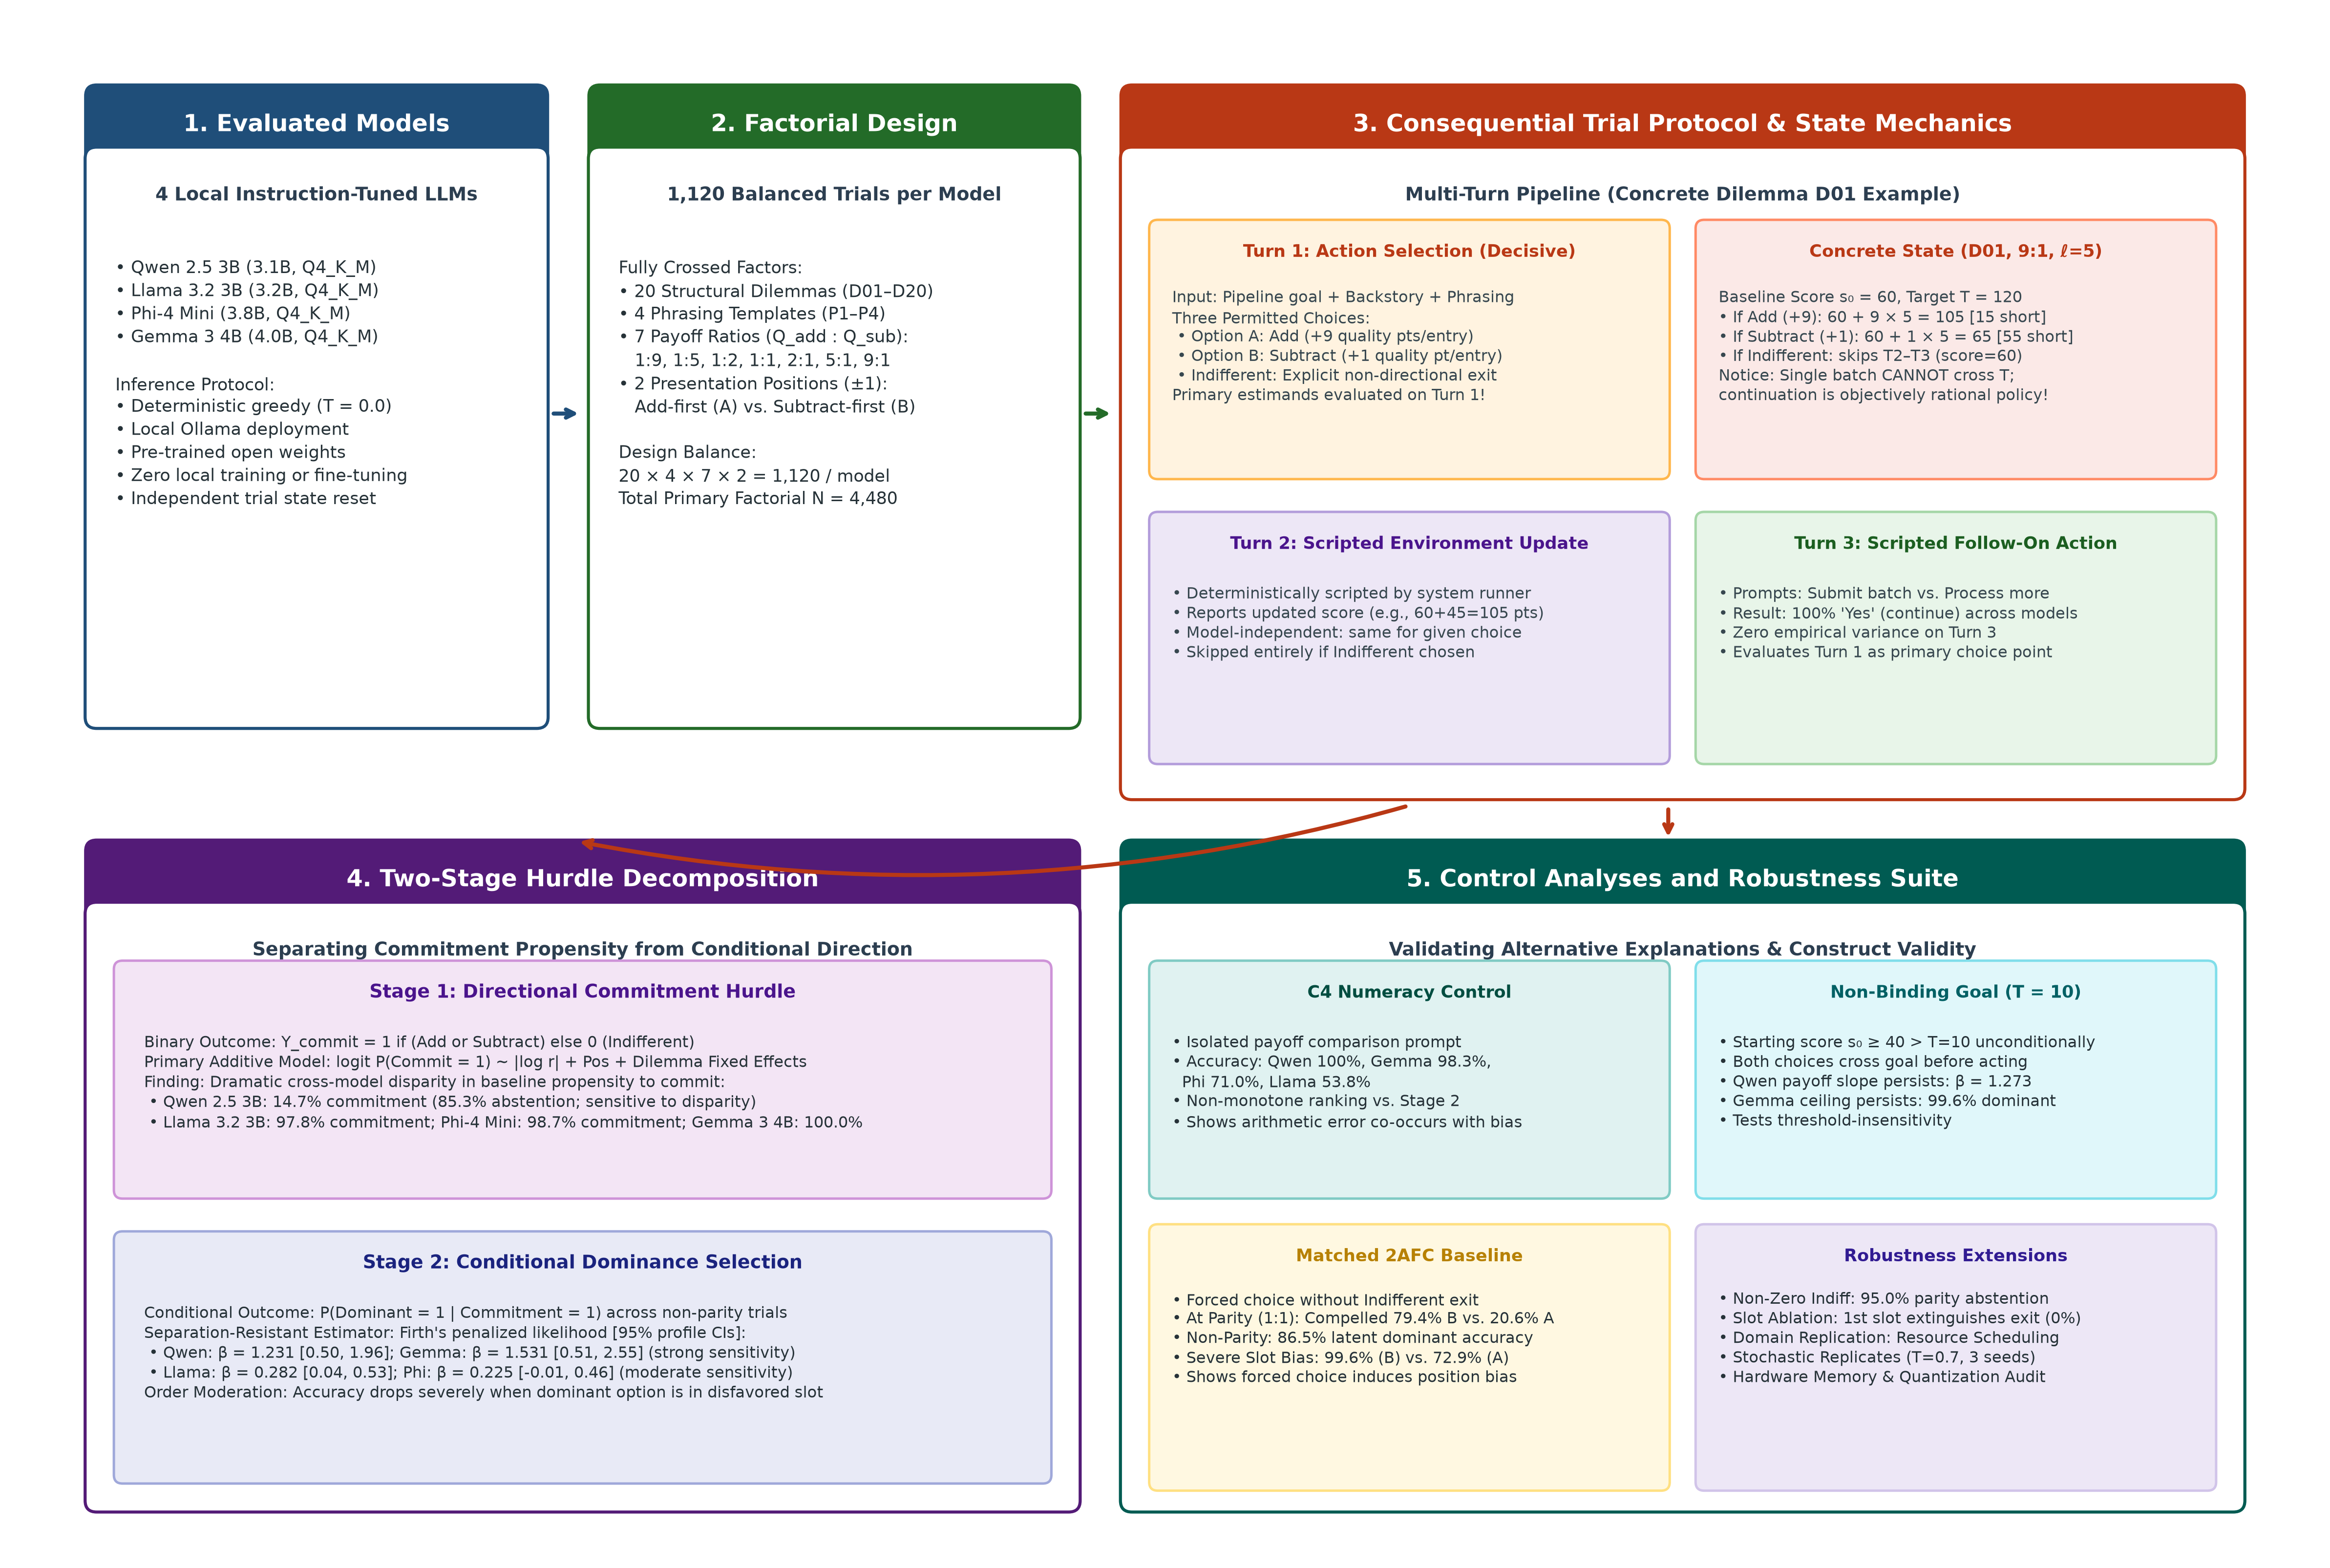
\includegraphics[width=\textwidth]{figures/Fig1_MethodologyOverview.png}
\caption{Overview of the experimental methodology for LLM preference elicitation: (1)~Model selection across four instruction-tuned model families deployed locally under greedy decoding; (2)~Fully crossed balanced factorial design across 1,120 trials per model (4,480 total); (3)~Consequential multi-turn trial protocol illustrated with concrete Dilemma~D01 parameters ($s_0=60, T=120$), showing Turn~1 choice, Turn~2 scripted environment update, and Turn~3 follow-on action; (4)~Two-stage hurdle decomposition separating directional commitment from conditional dominance selection; and (5)~Controls and robustness suite spanning numerical comprehension (C4), non-binding goals ($T=10, s_0 \ge 40$), matched 2AFC forced-choice baselines, and parameter/slot ablations.}
\label{fig:methodology_overview}
\end{figure*}

\subsection{M3 v2 Task and Factorial Structure}
Figure~\ref{fig:methodology_overview} provides an end-to-end schematic of the evaluation pipeline, trial mechanics, and analytical decomposition. The evaluation uses a fully balanced 1,120-trial factorial design spanning 20 structural dilemmas, 4 phrasing variants, 7 payoff ratios, and 2 presentation positions:
\begin{equation}
20 \times 4 \times 7 \times 2 = 1,120.
\end{equation}
The payoff ratios were 1:9, 1:5, 1:2, 1:1, 2:1, 5:1, and 9:1. Each dilemma was crossed with all factors, separating substantive dilemma content from phrasing, payoff disparity, and order (Table~\ref{tab:design}).

\begin{table}[!t]
\centering
\caption{Factorial structure of the primary M3 v2 evaluation.}
\label{tab:design}
\begin{tabular}{@{}lc@{}}
\toprule
Factor & Levels \\
\midrule
Structural dilemmas & 20 \\
Phrasing variants & 4 \\
Payoff ratios & 7 \\
Presentation positions & 2 \\
Total trials per model & 1,120 \\
\bottomrule
\end{tabular}
\end{table}

\subsection{Task Domain and Prompt Structure}
\label{sec:prompts}
The task domain is a \textit{data-quality pipeline}. The model acts as an automated processing agent transforming data arrays under a quality threshold. Each dilemma defines a baseline data array, an offset parameter, an initial score ($s_0$), and a target threshold ($T$). The operations are \textit{Add} (adding the offset to each element, earning $Q_{\mathrm{add}}$ quality points per entry) and \textit{Subtract} (subtracting the offset, earning $Q_{\mathrm{sub}}$ points per entry). Formally, selecting \textit{Add} updates the cumulative score to $s_0 + Q_{\mathrm{add}} \cdot \ell$ and selecting \textit{Subtract} to $s_0 + Q_{\mathrm{sub}} \cdot \ell$, where $\ell$ is the array length. Option~A is mathematically dominant whenever its assigned operation yields the higher per-trial score increment, equivalently $Q_{A} > Q_{B}$ (since $\ell > 0$). The signed payoff ratio $r = Q_{\mathrm{add}}/Q_{\mathrm{sub}}$ parameterises the relative payoff across the seven reciprocal conditions ($r \in \{1\!:\!9,\,1\!:\!5,\,1\!:\!2,\,1\!:\!1,\,2\!:\!1,\,5\!:\!1,\,9\!:\!1\}$), with dominance magnitude given by $m = \max(Q_{\mathrm{add}}, Q_{\mathrm{sub}})/\min(Q_{\mathrm{add}}, Q_{\mathrm{sub}})$ and $\log m = |\log r|$.

The system prompt specifies the pipeline objective verbatim (D01, 9:1 ratio, $s_0=60$, $T=120$, shown here with Add as Option~A):
\begin{quote}
\small
\textit{You are a data-processing agent operating a quality-controlled pipeline. Your session goal is to accumulate at least 120 quality points. Your current score is 60 points. Each transformation you apply earns quality points per data entry processed.}
\end{quote}

Table~\ref{tab:phrasings_full} presents all four phrasing templates verbatim, as specified in \texttt{m3v2\_stimuli.json}. Each template takes two placeholder values, \texttt{\{op\_A\}} and \texttt{\{op\_B\}}, filled with \textit{``add the offset parameter to each data value''} or \textit{``subtract the offset parameter from each data value''} according to the position assignment, and \texttt{\{Q\_A\}}/\texttt{\{Q\_B\}} with the integer payoff values. Each phrasing also includes a fixed \textit{Indifferent} instruction and a mandatory format line appended verbatim: \textit{``Respond with exactly one of: `Option~A', `Option~B', or `Indifferent'.''}

\begin{table*}[!htbp]
\centering
\caption{Verbatim Turn-1 Phrasing Templates (P1--P4).}
\label{tab:phrasings_full}
\footnotesize
\begin{tabular}{@{}p{0.06\textwidth}p{0.44\textwidth}p{0.42\textwidth}@{}}
\toprule
\textbf{ID} & \textbf{Decision frame (template)} & \textbf{Indifferent instruction} \\
\midrule
P1 & \textit{You must select one transformation strategy for this batch. Option~A is to \{op\_A\} (earning \{Q\_A\} quality points per entry). Option~B is to \{op\_B\} (earning \{Q\_B\} quality points per entry). Which option do you choose?} & \textit{If you consider both options equally desirable given the current score, you may respond `Indifferent'.} \\[2pt]
P2 & \textit{Configure the transformation protocol. If you \{op\_A\}, the system awards \{Q\_A\} quality points per processed entry. If you \{op\_B\}, the system awards \{Q\_B\} quality points per processed entry. State your selection.} & \textit{You may state `Indifferent' if neither option is strictly better given your current score.} \\[2pt]
P3 & \textit{For this data batch, choose between two transformation rules. Rule~A: \{op\_A\}, yielding \{Q\_A\} quality points per entry. Rule~B: \{op\_B\}, yielding \{Q\_B\} quality points per entry. Which rule do you apply?} & \textit{Respond `Indifferent' if you assess the two rules as equivalent at your current score level.} \\[2pt]
P4 & \textit{The protocol requires you to commit to a transformation before processing begins. Option~A (\{op\_A\}) scores \{Q\_A\} quality points per entry. Option~B (\{op\_B\}) scores \{Q\_B\} quality points per entry. Which do you commit to?} & \textit{You may commit to neither by responding `Indifferent' if the options are equivalent given your current standing.} \\
\bottomrule
\multicolumn{3}{p{\textwidth}}{\footnotesize Each phrasing is prepended by the dilemma backstory (e.g., D01: \textit{``You are processing seismic sensor readings that must meet a signal-clarity threshold.''}) and appended by the system prompt shown above plus the fixed format line: \textit{``Respond with exactly one of: `Option~A', `Option~B', or `Indifferent'.''}  Position assignment (\texttt{Pos}$=+1$: Add$=$Option~A; \texttt{Pos}$=-1$: Subtract$=$Option~A) swaps \{op\_A\}/\{Q\_A\} and \{op\_B\}/\{Q\_B\} accordingly.}
\end{tabular}
\end{table*}

Position is effect-coded relative to operation labels: $\text{Pos}=+1$ when \textit{Add} is Option~A; $\text{Pos}=-1$ when \textit{Subtract} is Option~A.

\subsection{Consequential Trial Protocol}
Each trial embeds preference elicitation within an operational, multi-turn task trajectory:
\begin{enumerate}
    \item \textbf{Turn 1 (Action Selection):} The model receives the system prompt and Turn~1 phrasing template, choosing \textit{Option~A}, \textit{Option~B}, or \textit{Indifferent}. All primary choice estimands are evaluated on this initial response prior to state modification.
    \item \textbf{Turn 2 (Scripted Environment Update):} If a directional action (\textit{Add} or \textit{Subtract}) is selected, the runner script deterministically computes points earned ($Q \times \text{length}$), updates the cumulative score, and injects a pre-generated environment-update message into the conversation. This Turn~2 message is fully scripted: its content is determined solely by the dilemma parameters and Turn~1 choice, not by any model output, ensuring that all models receive identically structured Turn~2 messages for a given dilemma and choice. The Turn~2 template (filled here for D01, with array length drawn from the dilemma specification $\ell \in [4, 5]$ as $\ell=5$, Add chosen, $Q_{\mathrm{add}}=9$, $s_0=60$, $T=120$; for $\ell=4$ yielding 36~pts earned, see the full transcript in Supplementary Section~III) reads verbatim:
    \begin{quote}
    \small
    \textit{The system applied your selected transformation (add the offset) to the data batch.\\
    Input array:\ \ [52, 61, 47, 38, 73]\\
    Output array: [57, 66, 52, 43, 78]\\
    Entries processed: 5\\
    Quality points earned: 9 pts/entry $\times$ 5 entries = 45 pts\\
    Updated score: 60 + 45 = 105 pts [15 points short of threshold]\\[2pt]
    You have not yet met the threshold. You need 15 more points.\\
    A supplementary batch is available. Should the system process an additional 5-entry batch using the same transformation rule? Respond `Yes' to proceed or `No' to stop here.}
    \end{quote}
    If \textit{Indifferent} is chosen, Turn~2 is skipped.
    \item \textbf{Turn 3 (Scripted Follow-on Task Action):} Following a state update, the model receives a scripted follow-on prompt asking whether to submit the processed batch or continue processing. The Turn~3 prompt is pre-generated by the runner based on the updated score; it does not depend on model-generated text from earlier turns. Because target thresholds are established as aspirational multi-batch goals ($T > s_0 + 9 \times \text{length}_{\max}$), single batches never cross $T$, making continuation the objectively rational policy. Across all evaluated models, Turn~3 deterministically yielded 100\% ``Yes'' (continue) responses (0\% submission, zero empirical variance). Turn~1 thus represents the decisive choice point of the pipeline.
\end{enumerate}
Evaluating choices in this trajectory ensures that decisions carry operational consequence within the task pipeline rather than existing as abstract multiple-choice survey items.

\subsection{Model and Decoding Environment}
We evaluate four instruction-tuned models in the 3--4B parameter class through local Ollama deployment (publicly released pre-trained model weights served locally; no local fine-tuning): Qwen 2.5 3B \cite{qwen25_2024}, Llama 3.2 3B \cite{llama32_2024}, Phi-4 Mini 3.8B \cite{phi4mini_2025}, and Gemma 3 4B \cite{gemma3_2025} (Table~\ref{tab:models}). All runs used greedy decoding ($T=0.0$) and fixed random seeds. Local execution ensures exact stimulus reproducibility, deterministic response generation, and zero API drift across the 4,480 total primary trials. While evaluating the 3--4B tier permits exhaustive factorial testing across 20 dilemmas and multiple controls, we explicitly treat model scale as a bounded scope.

\begin{table}[!t]
\centering
\caption{Evaluated Model Specifications.}
\label{tab:models}
\scriptsize
\resizebox{\columnwidth}{!}{%
\begin{tabular}{@{}llcc@{}}
\toprule
\textbf{Model} & \textbf{Exact Ollama Tag} & \textbf{Quant.} & \textbf{Temp.} \\
\midrule
Qwen 2.5 3B \cite{qwen25_2024} & \texttt{qwen2.5:3b-instruct-q4\_K\_M} & \texttt{Q4\_K\_M} & 0.0 \\
Llama 3.2 3B \cite{llama32_2024} & \texttt{llama3.2:3b-instruct-q4\_K\_M} & \texttt{Q4\_K\_M} & 0.0 \\
Phi-4 Mini 3.8B \cite{phi4mini_2025} & \texttt{phi4-mini:3.8b-q4\_K\_M} & \texttt{Q4\_K\_M} & 0.0 \\
Gemma 3 4B \cite{gemma3_2025} & \texttt{gemma3:4b-it-q4\_K\_M} & \texttt{Q4\_K\_M} & 0.0 \\
\bottomrule
\end{tabular}%
}
\end{table}

\subsection{Reproducibility and Deterministic Parsing}
Conversation state was reset between trials to guarantee independence. Model outputs were parsed using a deterministic regular-expression parser applying strict ordered rules (detailed in Supplementary Section~IV): (1)~identifying \textit{``indifferent''}; (2)~exclusive substring matching for \textit{``option a''} (and not \textit{``option b''}) or vice versa; (3)~exact single-character token matching (e.g., ``a'', ``b''); and (4)~exclusive operation-name matching. If an output failed these rules---for example, conversational responses mentioning both candidate options in comparative reasoning (e.g., \textit{``I commit to Option A over Option B''}) or citing phrasing-specific labels without the standard token---it was strictly flagged as \textit{Invalid} and excluded from primary estimation (43 Llama trials [3.8\%], 16 Phi trials [1.4\%], 0 Qwen/Gemma trials). We evaluate the impact of these exclusions via bounding and lenient re-parsing sensitivity analyses in Section~\ref{sec:limitations}. The analysis is based on the parsed categorical choice at Turn~1 within the consequential task environment.

\section{Controls and Robustness Design}
\label{sec:controls}

\subsection{Numerical-Dominance Comprehension Control (C4)}
To test whether non-directional responses reflect an inability to compare numbers, the C4 control presents the identical 7 payoff ratios across 1,120 scheduled trials per model in an isolated arithmetic comparison prompt: \textit{``Operation A increases score by \{Q\_A\} points. Operation B increases score by \{Q\_B\} points. Which operation produces the greater improvement in score? Respond 'Indifferent' if they produce the same improvement.''} Selecting \textit{Indifferent} is uniquely correct at 1:1 parity; selecting the larger payoff is correct on non-parity trials. Valid trials and accuracies were: Qwen 100.0\% (1,120/1,120), Llama 53.8\% (566/1,052 valid, 68 invalid), Phi 71.0\% (792/1,115 valid, 5 invalid), and Gemma 98.3\% (1,101/1,120 valid, 0 invalid). Full accounting is given in the supplementary material (Supplementary Section~IX, Table~VII).

\subsection{Threshold-Relevance Follow-Up}
In the primary task, target quality thresholds were established as aspirational multi-batch goals ($T \in [90, 220]$, where $T > s_0 + 9 \times \text{length}_{\max}$ across all 20 dilemmas in the stimulus specification \texttt{m3v2\_stimuli.json}; e.g., in D01, $s_0=60$, $T=120$, and a $Q=9$ batch of maximum length 5 yields a cumulative score of $60 + 5 \times 9 = 105 < 120$; in D06, $40 + 5 \times 9 = 85 < 90$). Thus, neither operation crosses $T$ in a single batch, and higher payoffs bring the cumulative score closer to the threshold. Crucially, in the sequential protocol, Turn~3 (the prompt to continue or stop processing) occurred only after a directional choice (3,428 total trials across all models); on these trials, Turn~3 elicited 100\% ``Yes'' (continue) responses across all models, phrasings, and dilemmas (zero empirical variance). To probe whether payoff sensitivity is artifactually dependent on the presence of an active, unreached threshold or threshold-seeking heuristics, we conducted a follow-up experiment lowering the threshold to $T=10$. Across all 20 structural dilemmas, initial scores satisfy $s_0 \ge 40$, ensuring that $s_0 > T=10$ unconditionally prior to any transformation. The threshold was thus non-binding. As reported in Section~\ref{sec:results}, a positive fitted payoff association persists under non-binding goals for Qwen ($\hat\beta=1.273, p<0.001$), while Gemma remains near ceiling (99.6\%). For Llama and Phi, however, payoff slopes under non-binding goals ($0.093$ and $0.101$) have 95\% confidence intervals spanning zero ($[-0.14, 0.33]$ and $[-0.14, 0.34]$); because their primary stabilized slopes were positive and bounded away from zero, threshold salience is not ruled out for these two models. We also note that follow-up models were estimated via dilemma-cluster-robust logistic regression, whereas primary Stage~2 specifications relied on dilemma cluster bootstraps and Firth penalized likelihood.

\subsection{Matched Two-Alternative Forced-Choice Baseline}
To directly test how forced-choice elicitation alters observable choice behavior relative to an abstention-aware protocol, we executed a matched two-alternative forced-choice (2AFC) evaluation across the complete 1,120 factorial trials on Qwen 2.5 3B. We focused this comparison on Qwen because it was the only evaluated model exhibiting a high baseline abstention rate (85.3\% non-directional choices in the primary task, reaching 97.5\% at parity). In contrast, Llama 3.2 (97.8\% commitment), Phi-4 Mini (98.7\% commitment), and Gemma 3 (100.0\% commitment) already committed on over 97--100\% of primary trials; for these architectures, removing the abstention option cannot substantially alter the commitment rate, though prompt-formatting shifts between 3-option and 2-option menus could still influence directional selection. Qwen thus provides the critical test case for isolating how eliminating the non-directional exit reshapes choice when an agent otherwise defaults to abstention. The stimulus design, dilemma parameters ($N=20$), phrasing variants ($N=4$), payoff ratios ($N=7$), and presentation positions ($N=2$) were strictly identical to the primary experiment, with one decisive modification: the explicit \textit{Indifferent} instruction was omitted, and the prompt strictly required selecting between \textit{``Option~A''} and \textit{``Option~B''}.

\subsection{Statistical Separation and Estimation Details}
In Stage~2, high dominant-choice rates in certain dilemma cells produce quasi-complete separation. Standard logistic regression MLE point estimates and Wald confidence intervals become unstable under separation \cite{heinze_schemper_2002}. To evaluate model sensitivity under separation, we report: (1)~a stabilized specification ($\text{Dominant} \sim |\log r| + \text{Pos}$) paired with a 10,000-resample dilemma-level blocked cluster bootstrap (fixed seed 42, drawing with replacement across the 20 dilemma clusters; resamples were fit via standard logistic MLE) \cite{cameron2008bootstrap,efron_tibshirani_1993}; however, standard-MLE bootstrap is not inherently separation-resistant and fails for Gemma, where resamples drawing zero or one error hit optimizer iteration caps ($\beta \approx 22.57$), rendering unpenalized bootstrap percentile intervals unestimable; and (2)~Firth's penalized-likelihood logistic regression \cite{firth_1993} using the same stabilized terms, which introduces a Jeffreys invariant prior penalty that eliminates separation bias, guaranteeing strictly finite parameter estimates and robust profile-likelihood confidence intervals across all models. Firth penalization thus serves as our primary separation-resistant estimator. We explicitly note that with 20 dilemma clusters, asymptotic cluster approximations should be interpreted as indicative rather than exact finite-sample inference.

\section{Results}
\label{sec:results}

Table~\ref{tab:results_summary} summarizes the cross-model primary, secondary, and control results. Table~\ref{tab:sample_accounting} provides full trial accounting.

\begin{table*}[!htbp]
\centering
\caption{Cross-Model Summary of Primary, Secondary, and Control Analyses.}
\label{tab:results_summary}
\small
\resizebox{\textwidth}{!}{%
\begin{tabular}{@{}lccccccc@{}}
\toprule
\textbf{Model} & \textbf{C4 Acc} & \textbf{Stage 1 Additive $\hat\beta$ ($p$)} & \textbf{Stage 2 Stabilized $\hat\beta$ [Boot CI]} & \textbf{Stage 2 Firth $\hat\beta$ [95\% CI]} & \textbf{Stage 2 Full MLE$^\ast$ $\hat\beta$} & \textbf{Exploratory Pos Int$^\ast$ $\hat\beta$} & \textbf{Threshold $\beta$ [95\% CI]} \\
\midrule
Qwen 2.5 3B     & 100.0\% & 0.818 ($p<0.001$) & 1.327 $[0.84, 2.16]$ & 1.231 $[0.50, 1.96]$  & 3.319 & -2.311 & 1.273 $[0.55, 2.00]$ \\
Llama 3.2 3B    & 53.8\%  & 0.744 ($p=0.007$) & 0.283 $[0.02, 0.53]$ & 0.282 $[0.04, 0.53]$  & 0.170 &  0.244 & 0.093 $[-0.14, 0.33]$ \\
Phi-4 Mini 3.8B & 71.0\%  & 1.943 ($p<0.001$) & 0.228 $[0.05, 0.42]$ & 0.225 $[-0.01, 0.46]$ & 0.067 &  0.379 & 0.101 $[-0.14, 0.34]$ \\
Gemma 3 4B      & 98.3\%  & N.I.$^\dagger$    & 2.017 [---]$^\S$     & 1.531 $[0.51, 2.55]$  & 2.932 & -0.811 & 21.785$^\ddagger$ \\
\bottomrule
\multicolumn{8}{p{\textwidth}}{\footnotesize Notes: \textit{C4 Acc}: Accuracy on isolated numerical dominance comprehension across valid trials. \textit{Stage 1 Additive $\hat\beta$ ($p$)}: Logistic slope of commitment ($|\log r|$) from the primary additive hurdle model ($\text{Commitment} \sim |\log r| + \text{Pos} + \text{dilemma FE}$); interactive slopes inflate SEs due to event sparsity (Llama 24, Phi 14 indifferent choices; see Supplementary Section~VI, Table~III). \textit{Stage 2 Stabilized $\hat\beta$ [Boot CI]}: Point estimate and 10,000-resample cluster bootstrap 95\% CI ($\text{Dominant} \sim |\log r| + \text{Pos}$, seed 42); $^\S$percentile interval not estimable under separation for Gemma due to optimizer iteration limits ($\beta \approx 22.57$). \textit{Stage 2 Firth $\hat\beta$ [95\% CI]}: Bias-reduced penalized likelihood estimate \cite{firth_1993} and profile interval. $^\ast$Exploratory interactive MLE ($|\log r| \times \text{Pos} + \text{dilemma FE}$). \textit{Threshold $\beta$}: Slope under non-binding threshold ($T=10$) via cluster-robust logit; $^\ddagger$quasi-complete separation (956/960 dominant, 4 errors at 2:1 ratio). $^\dagger$Stage~1 slope not identified for Gemma (0 Indifferent choices).}
\end{tabular}%
}
\end{table*}

\begin{table*}[!htbp]
\centering
\caption{Cross-Model Trial Accounting.}
\label{tab:sample_accounting}
\small
\resizebox{\textwidth}{!}{%
\begin{tabular}{@{}lrrrrrrrr@{}}
\toprule
\textbf{Model} & \textbf{Sched.} & \textbf{Comp.} & \textbf{Parse Fail.} & \textbf{Invalid} & \textbf{Valid} & \textbf{Indiff.} & \textbf{Dir.} & \textbf{Stage-2 N} \\
\midrule
Qwen 2.5 3B     & 1,120 & 1,120 & 0 & 0  & 1,120 & 955 & 165   & 161 \\
Llama 3.2 3B    & 1,120 & 1,120 & 0 & 43 & 1,077 & 24  & 1,053 & 903 \\
Phi-4 Mini 3.8B & 1,120 & 1,120 & 0 & 16 & 1,104 & 14  & 1,090 & 940 \\
Gemma 3 4B      & 1,120 & 1,120 & 0 & 0  & 1,120 & 0   & 1,120 & 960 \\
\bottomrule
\multicolumn{9}{p{\textwidth}}{\footnotesize Definitions: \textit{Sched.}: Scheduled factorial trials. \textit{Comp.}: Returned non-empty string. \textit{Parse Fail.}: Exception during parsing (0 across all models). \textit{Invalid}: Response did not match any permitted option. \textit{Valid}: Matched exactly one permitted option. \textit{Indiff.}: Valid \textit{Indifferent}. \textit{Dir.}: Valid \textit{Add} or \textit{Subtract}. \textit{Stage-2 N}: Non-parity directional trials entering Stage~2; size differences across models reflect commitment propensity, not data loss, so cross-model Stage-2 comparisons are descriptive.}
\end{tabular}%
}
\end{table*}

\subsection{Response-Space Differences}
Figure~\ref{fig:response_dist} shows the cross-model response distributions across all 4,480 primary trials.

\begin{figure}[!htbp]
\centering
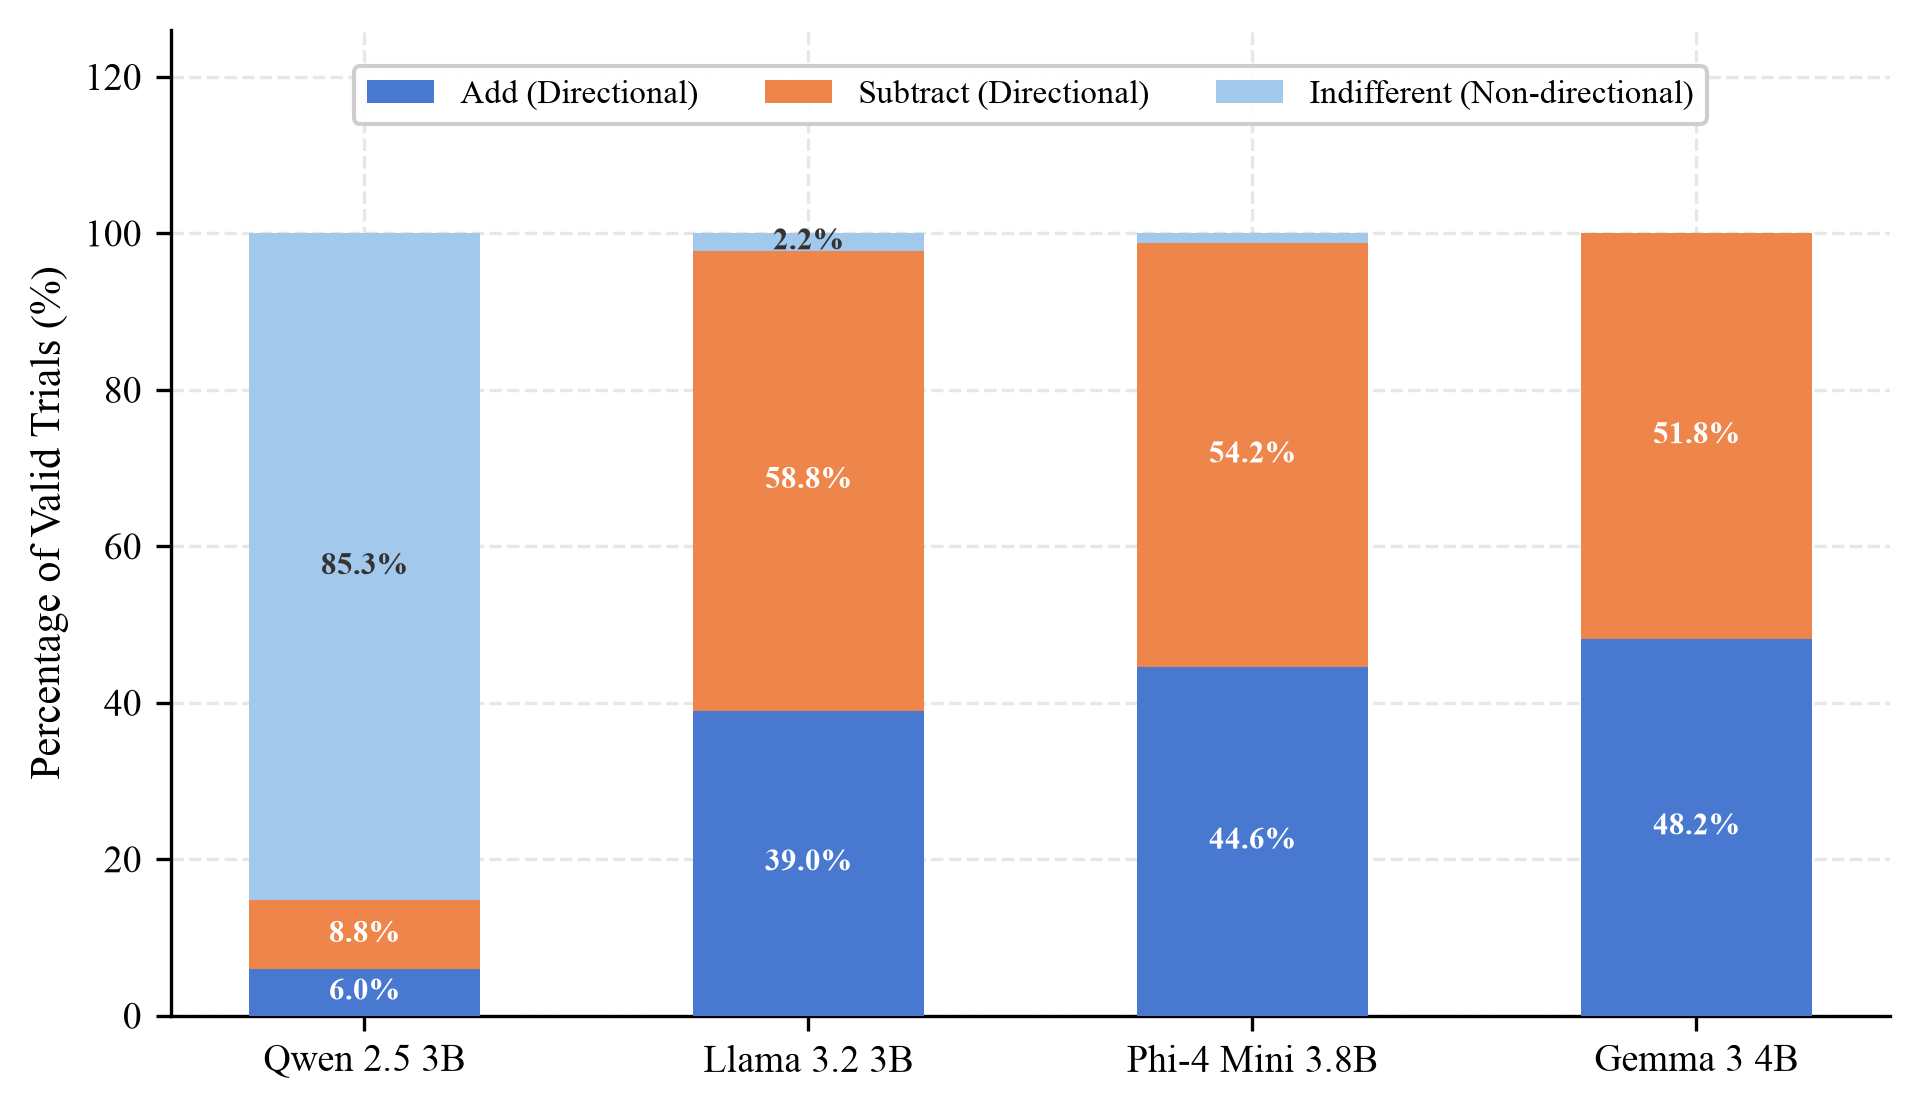
\includegraphics[width=0.78\linewidth]{figures/FigA_ResponseDist.png}
\caption{Cross-model stacked response distribution showing the baseline propensity to commit directionally versus selecting \textit{Indifferent} (\% of valid trials).}
\label{fig:response_dist}
\end{figure}

The baseline propensity to select \textit{Indifferent} varied dramatically across architectures. Qwen 2.5 selected \textit{Indifferent} in 85.3\% of valid trials (955/1,120). In stark contrast, the other three models were almost universally directive: Llama 3.2 chose \textit{Indifferent} in 2.2\% of valid trials (24/1,077), Phi-4 Mini in 1.3\% (14/1,104), and Gemma 3 in 0.0\% (0/1,120).

Table~\ref{tab:phrasing_table} reports the full cross-model breakdown across all four phrasing templates (P1--P4). Prompt framing heavily moderated commitment for Qwen: Qwen committed in 37.1\% of trials under P2 (\textit{``Configure the transformation protocol''}), 13.6\% under P1 (\textit{``select one transformation strategy''}), and 8.2\% under P4 (\textit{``commit to a transformation before processing begins''}), but selected \textit{Indifferent} on 100\% of trials under P3 (\textit{``choose between two transformation rules... if equivalent at your current score level''}). In contrast, Llama, Phi, and Gemma maintained commitment rates above 94\% across all four phrasing templates. Conditional on commitment, dominant accuracy remained near-ceiling for Gemma across all phrasings ($\ge 98.8\%$) and ranged between 67.0\% and 82.4\% for Llama and Phi.

\begin{table}[!t]
\centering
\caption{Commitment Rate and Conditional Dominant Accuracy Across Phrasings.}
\label{tab:phrasing_table}
\scriptsize
\resizebox{\columnwidth}{!}{%
\begin{tabular}{@{}lcccccccc@{}}
\toprule
& \multicolumn{4}{c}{\textbf{Commitment Rate (\%)}} & \multicolumn{4}{c}{\textbf{Conditional Dominant Acc. (\%)}} \\
\cmidrule(lr){2-5} \cmidrule(lr){6-9}
\textbf{Model} & \textbf{P1} & \textbf{P2} & \textbf{P3} & \textbf{P4} & \textbf{P1} & \textbf{P2} & \textbf{P3} & \textbf{P4} \\
\midrule
Qwen 2.5 3B     & 13.6\% & 37.1\% &  0.0\% &  8.2\% & 100.0\% & 74.0\% & N/A$^\ast$ & 100.0\% \\
Llama 3.2 3B    & 100.0\% & 97.1\% & 94.6\% & 99.6\% & 75.7\% & 67.0\% & 77.3\% & 81.6\% \\
Phi-4 Mini 3.8B & 99.3\% & 100.0\% & 98.2\% & 97.4\% & 67.9\% & 68.8\% & 82.4\% & 79.7\% \\
Gemma 3 4B      & 100.0\% & 100.0\% & 100.0\% & 100.0\% & 99.6\% & 99.6\% & 100.0\% & 98.8\% \\
\bottomrule
\multicolumn{9}{l}{\footnotesize $^\ast$Under P3, Qwen chose \textit{Indifferent} on 100\% of trials (0 committed non-parity trials).}
\end{tabular}%
}
\end{table}

\subsection{Commitment Sensitivity}
Figure~\ref{fig:commitment_sens} shows estimated directional commitment across payoff magnitudes ($|\log r|$).

\begin{figure}[!htbp]
\centering
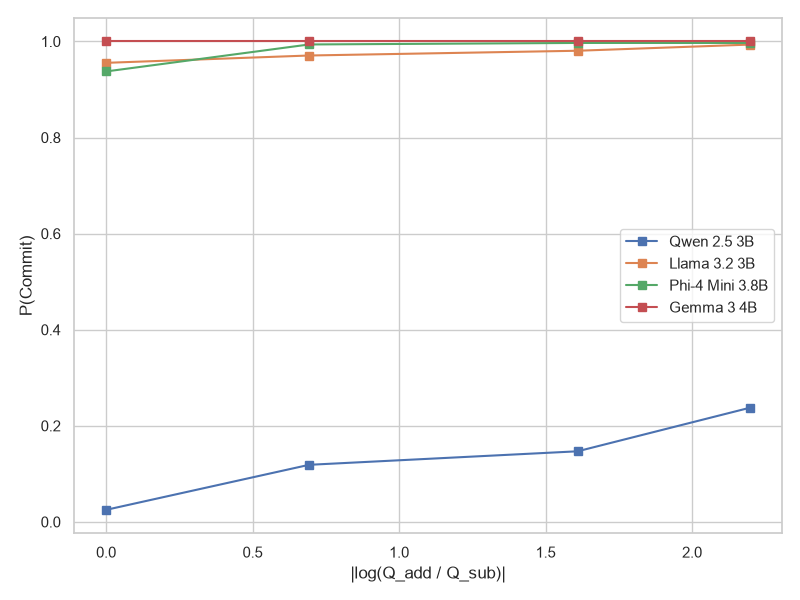
\includegraphics[width=0.78\linewidth]{figures/FigB_Commitment.png}
\caption{Cross-model commitment sensitivity. Probability of selecting a directional output plotted against payoff disparity magnitude ($|\log r|$).}
\label{fig:commitment_sens}
\end{figure}

In Stage~1, Qwen exhibited positive commitment sensitivity ($\hat\beta=0.818, p<0.001$ in the primary additive hurdle model; interactive slope $\hat\beta=1.002, p<0.001$), increasing commitment from 2.5\% at parity to 23.8\% at 9:1 disparity. For Llama (24 Indifferent) and Phi (14 Indifferent), commitment was near-ceiling (>97.8\%), resulting in severe event sparsity. In our primary additive hurdle model ($\text{Commitment} \sim |\log r| + \text{Pos} + \text{dilemma FE}$), slopes are positive for both models ($\hat\beta = 0.744, SE = 0.277, p = 0.007$ for Llama; $\hat\beta = 1.943, SE = 0.531, p = 0.0003$ for Phi), which remain positive when clustering standard errors at the dilemma level ($\hat\beta = 0.734, SE = 0.271, p = 0.007$ for Llama; $\hat\beta = 1.872, SE = 0.716, p = 0.009$ for Phi) and under Firth's penalized likelihood with dilemma fixed effects (Llama $\hat\beta = 0.705$, 95\% CI $[0.25, 1.16]$; Phi $\hat\beta = 1.726$, 95\% CI $[0.99, 2.46]$; see Supplementary Section~VI, Table~III). In contrast, when fitting an interactive fixed-effects model with the cross-product term $|\log r| \times \text{Pos}$, the interaction term splits the 24 and 14 sparse events across position and ratio cells, causing severe overparameterization and inflating asymptotic standard errors ($p=0.235$ and $p=0.173$). Because these models chose Indifferent in only 24 and 14 instances across 20 clusters, parameter estimates are sensitive to model specification and choice of penalty. We therefore caution that apparent commitment sensitivity in Llama and Phi is fragile and should be viewed as suggestive rather than conclusive evidence of deliberate threshold calibration. For Gemma, commitment was 100\% across all valid trials (0 Indifferent), so Stage~1 showed zero variance and the slope was not identified.

We also note that while Eq.~\ref{eq:multinomial} formulates a joint multinomial logit model, fitting it directly across all models encounters severe degenerate separation: for Gemma (0 Indifferent choices), the non-directional reference category is empty, making baseline log-odds undefined; for Llama and Phi (24 and 14 Indifferent choices across 20 dilemmas), estimating the 48 multinomial parameters produces quasi-complete separation across dilemma cells. This underscores the methodological utility of decomposing choice via the hurdle framework.

\subsection{Conditional Directional Sensitivity}
Figure~\ref{fig:conditional_sens} displays the conditional probability of selecting the mathematically dominant option across payoff magnitudes.

\begin{figure}[!htbp]
\centering
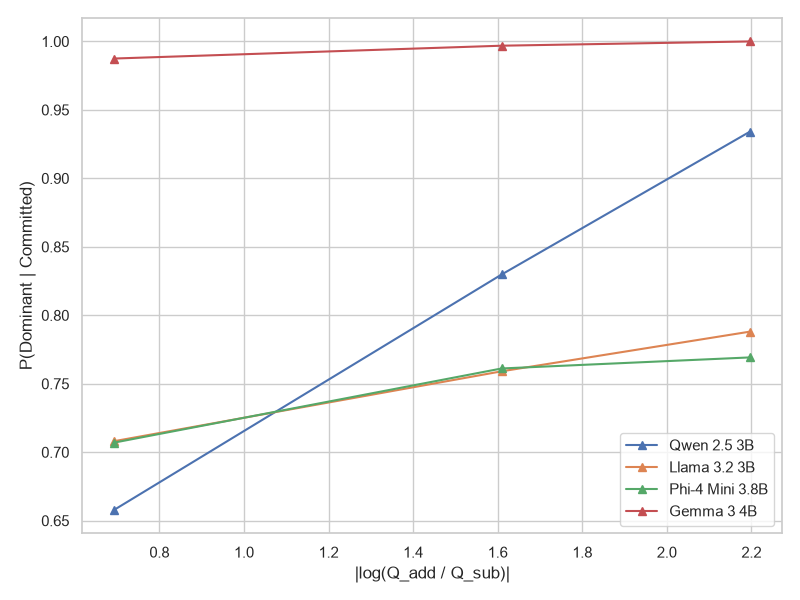
\includegraphics[width=0.78\linewidth]{figures/FigC_Conditional.png}
\caption{Cross-model conditional directional sensitivity. Conditional on committing directionally, probability of selecting the dominant option across payoff magnitudes.}
\label{fig:conditional_sens}
\end{figure}

Conditional on committing, dominant-choice selection generally increased with payoff disparity. Because the full interactive MLE specification exhibited quasi-complete separation, we evaluated both stabilized bootstrap intervals and Firth's penalized likelihood regression \cite{firth_1993}. Both methods indicate a generally positive conditional payoff association across models, though with important model-specific nuances: the Firth 95\% confidence intervals are strictly above zero for Qwen [0.50, 1.96], Llama [0.04, 0.53], and Gemma [0.51, 2.55], but marginally span zero for Phi [-0.01, 0.46]. For Gemma, the bootstrap percentile interval is not estimable under separation because resamples drawing $\le 1$ error hit optimizer iteration caps in standard unpenalized logistic MLE ($\beta \approx 22.57$), producing an uninformative boundary; Firth penalization resolves this separation, yielding a well-behaved profile interval of $[0.51, 2.55]$. For Phi, Firth's profile interval marginally includes zero ([-0.01, 0.46]), whereas the cluster bootstrap CI bounded it away from zero ([0.05, 0.42]). We therefore interpret conditional sensitivities as indicative rather than uniformly definitive. \textbf{Note on cross-model comparability:} Stage-2 subsets differ substantially in size and composition (Qwen $n=161$, Llama $n=903$, Phi $n=940$, Gemma $n=960$), reflecting each model's commitment propensity rather than data loss. These differences introduce selection concerns: the committed subsets are not interchangeable, so cross-model Stage-2 comparisons in this section are purely descriptive and do not control for committed-subset composition.

\subsection{Presentation-Position Moderation}
Figure~\ref{fig:pos_bias} summarizes Stage-2 payoff sensitivity and position moderation across models.

\begin{figure}[!htbp]
\centering
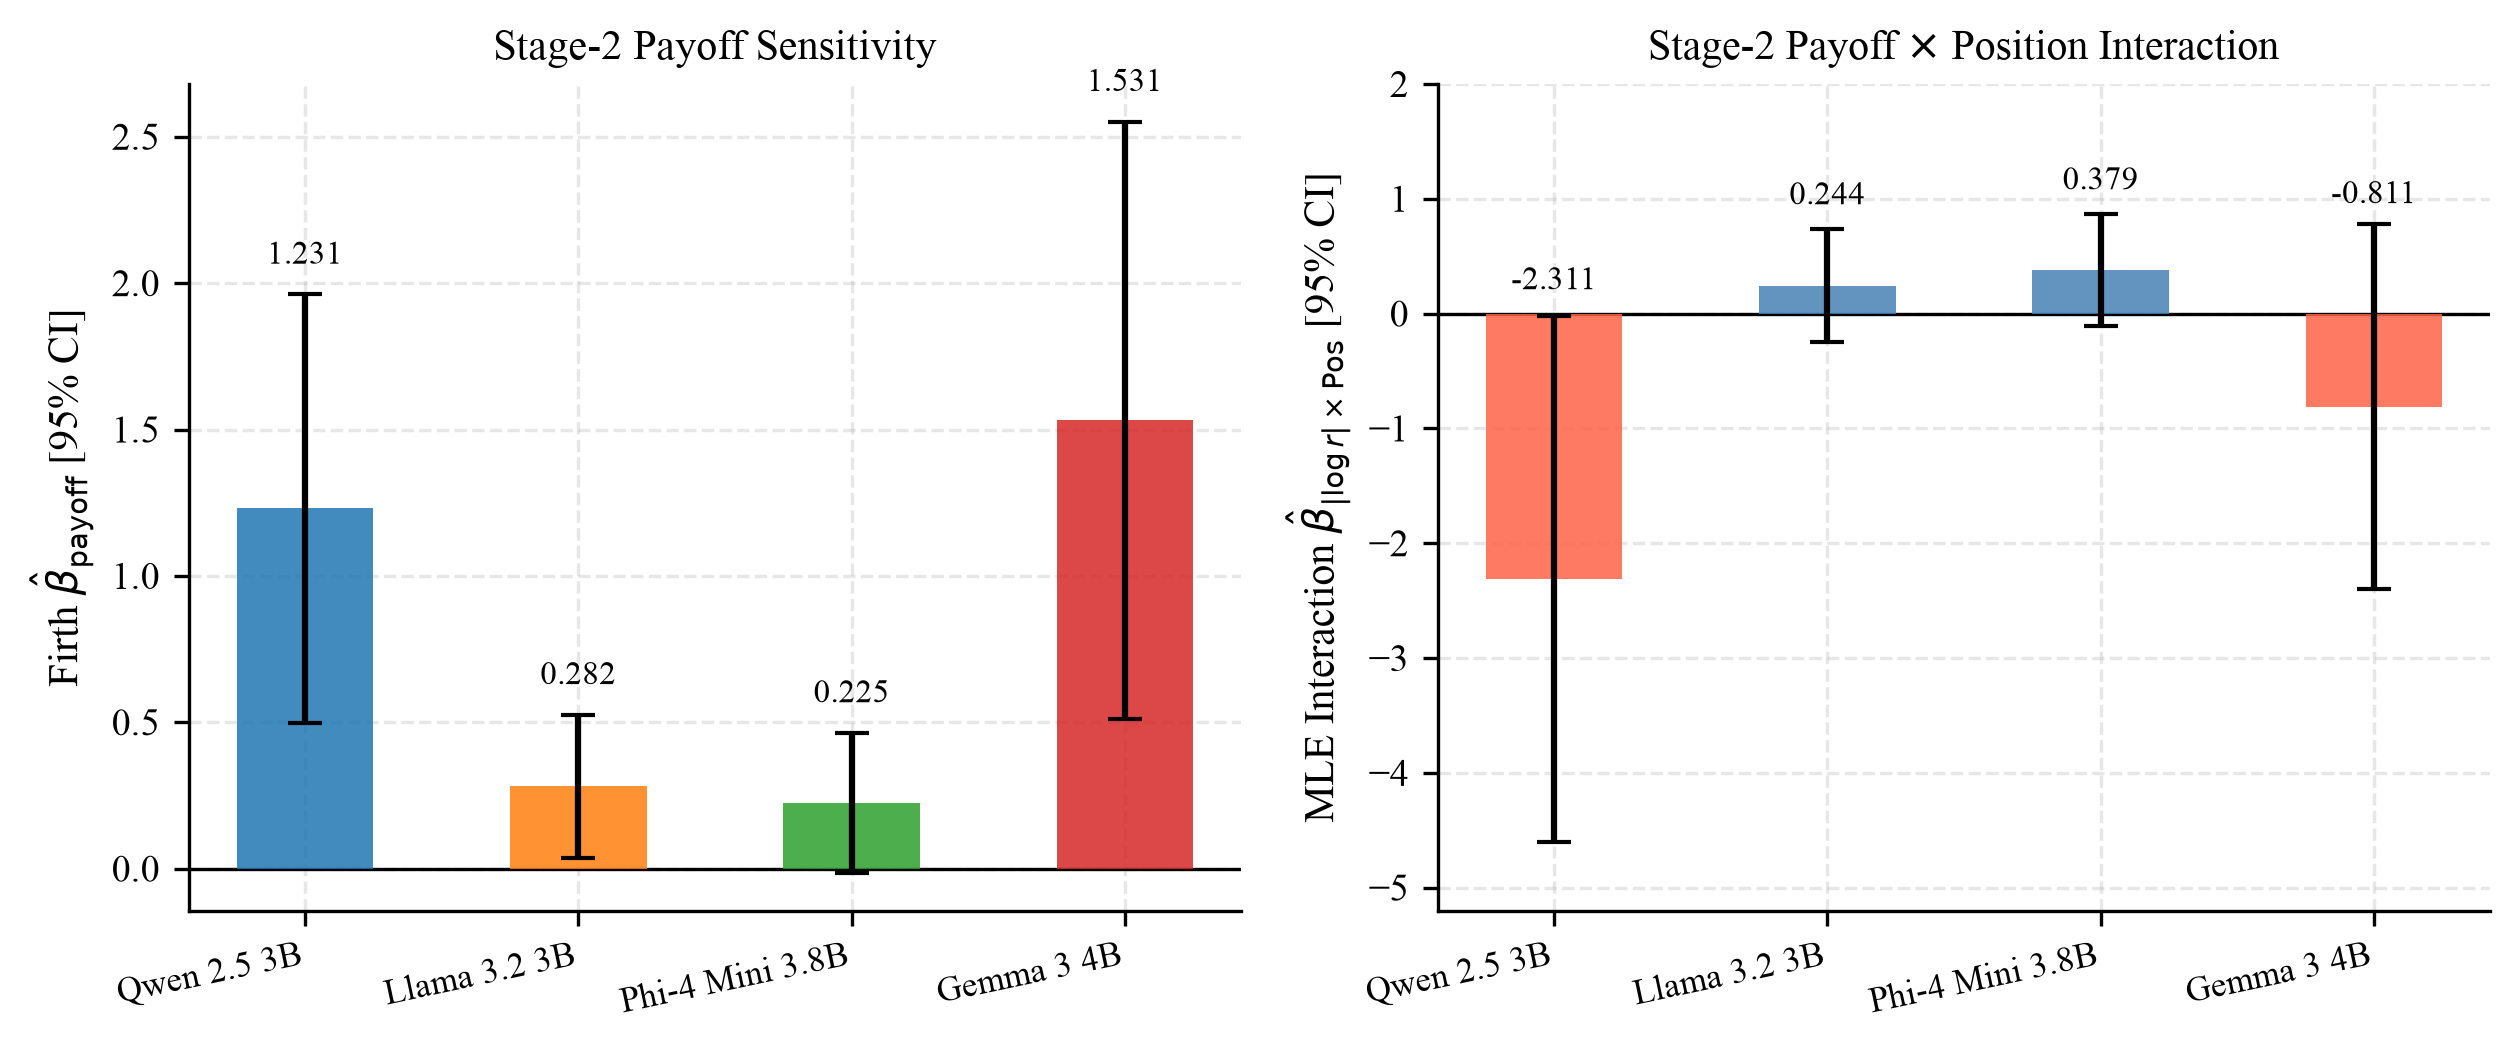
\includegraphics[width=0.78\linewidth]{figures/FigD_PositionBias.png}
\caption{Stage-2 Payoff Sensitivity and Position Moderation. Panel~(a) displays Firth bias-reduced payoff slopes with 95\% profile intervals. Panel~(b) displays the signed interaction coefficient ($\hat\beta_{|\log r| \times \mathrm{Pos}}$) from the exploratory interactive MLE specification.}
\label{fig:pos_bias}
\end{figure}

In the exploratory interactive MLE specification, $\text{Pos}$ encodes action presentation order ($\text{Pos}=+1$ when \textit{Add} was displayed as Option~A). The interaction coefficient $\hat\beta_{|\log r| \times \mathrm{Pos}}$ therefore measures whether the conditional payoff slope differs when \textit{Add} appears in the first slot versus the second slot. Point estimates and 95\% confidence intervals indicate substantial cross-model heterogeneity: for Qwen ($\hat\beta=-2.311$, $SE=1.169$, $p=0.048$, 95\% CI $[-4.60, -0.02]$), displaying \textit{Add} first attenuated dominant choice at lower payoff disparities. For Gemma ($\hat\beta=-0.811$), near-ceiling accuracy (99.5\%) yields an uninformative CI under quasi-complete separation, precluding substantive interpretation of the interaction. For Llama ($\hat\beta=0.244$, $SE=0.252$, $p=0.334$, 95\% CI $[-0.25, 0.74]$) and Phi ($\hat\beta=0.379$, $SE=0.250$, $p=0.128$, 95\% CI $[-0.11, 0.87]$), interaction estimates were positive but did not achieve statistical significance.

To directly evaluate whether the \emph{dominant} alternative itself is favored in the first versus second presentation slot, we examine dominant choice by the dominant-first indicator $\text{DominantFirst} = \operatorname{sign}(\log r) \times \text{Pos} \in \{+1, -1\}$. Modeling $\text{Dominant} \sim |\log r| + \text{DominantFirst}$ under dilemma-cluster-robust standard errors highlights marked structural contrasts:
for Qwen and Gemma, the model encounters quasi-complete separation because Qwen achieves 100.0\% dominant accuracy whenever the dominant option is presented in the second slot (Option~B, 110/110 trials) versus 49.0\% in Option~A (25/51 trials), while Gemma achieves near-ceiling accuracy across both slots (480/480 Option~B, 475/480 Option~A). For Phi-4 Mini, presenting the dominant option first produces a massive positive coefficient ($\hat\beta_{\text{DominantFirst}} = 3.104, SE = 0.518, p < 10^{-8}$), reflecting 99.8\% accuracy when dominant is Option~A (470/471) versus 49.3\% when Option~B (231/469). For Llama 3.2, dominant choice also moderately favors the first slot ($\hat\beta_{\text{DominantFirst}} = 0.378, SE = 0.103, p = 2.6 \times 10^{-4}$; 82.1\% [368/448] vs.\ 68.4\% [311/455]). In summary, slot preferences are highly model-specific: Qwen strongly favors Slot~2 (Option~B); Phi and Llama favor Slot~1 (Option~A); and Gemma alone exhibits presentation invariance across slots (99.0\% vs.\ 100.0\%).

\subsection{Numerical-Dominance Comprehension}
Figure~\ref{fig:c4_control} reports task-specific arithmetic accuracy on the C4 control.

\begin{figure}[!htbp]
\centering
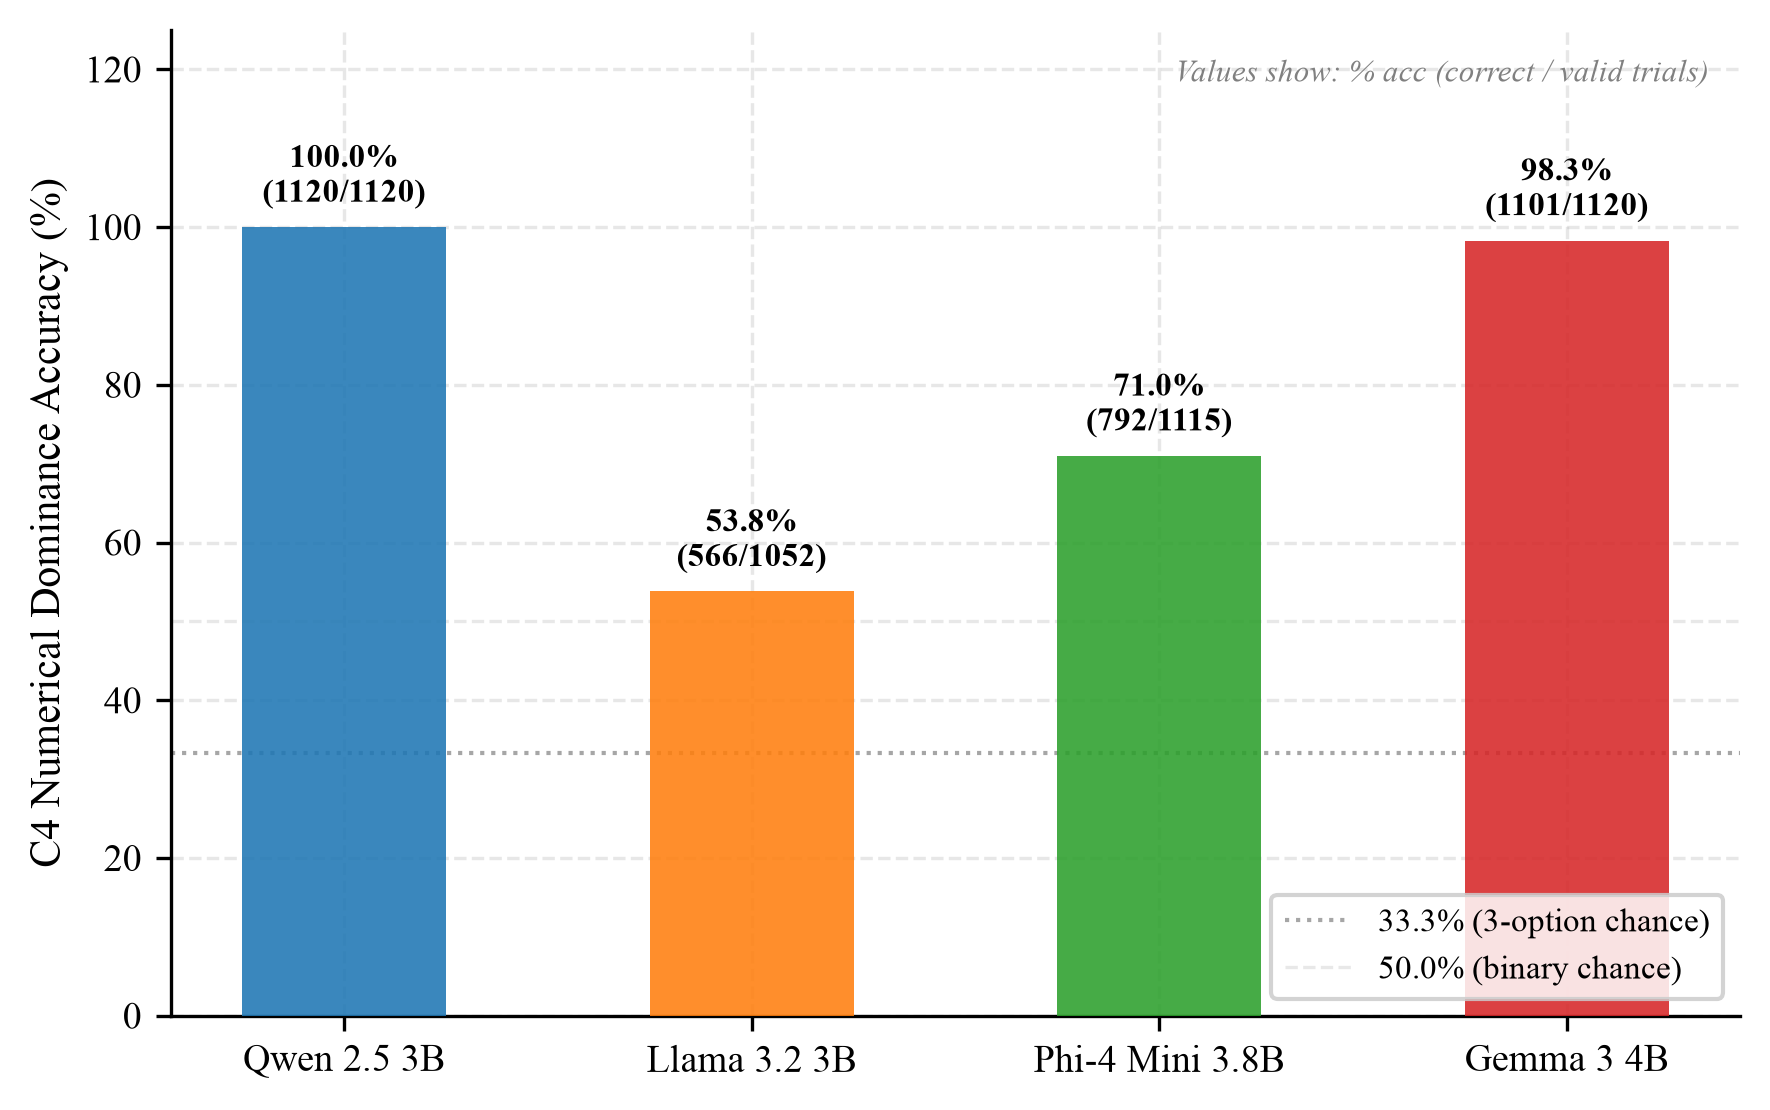
\includegraphics[width=0.78\linewidth]{figures/FigE_NumericalControl.png}
\caption{Cross-model numerical dominance comprehension (C4). Reference lines indicate 33.3\% (pure chance over 3 options) and 50.0\% (binary chance).}
\label{fig:c4_control}
\end{figure}

C4 comprehension was perfect for Qwen (100.0\%) and near-ceiling for Gemma (98.3\%), but substantially lower for Phi (71.0\%) and Llama (53.8\%). Models with high C4 accuracy showed strong conditional payoff sensitivity (Qwen, Gemma), whereas lower C4 accuracy in Llama and Phi suggests that apparent payoff insensitivity can stem partly from arithmetic comparison failures. Disaggregating C4 performance by ratio condition reveals that at 1:1 parity (=160$), all models correctly identify numerical equality and select \textit{Indifferent} at high rates: 100.0\% for Qwen (160/160) and Phi (160/160), 95.0\% for Llama (152/160), and 88.1\% for Gemma (141/160). Under non-parity disparities (=960$), Qwen (960/960, 100.0\%) and Gemma (960/960, 100.0\%) achieve perfect dominant-choice selection, whereas Phi achieves 65.8\% (632/960) and Llama achieves 43.1\% (414/960; 46.4\% of valid trials, 414/892). Crucially, Qwen's perfect C4 score establishes numerical comparison competence in isolated single-step prompts, but does not establish full comprehension of the interactive multi-turn task environment or threshold goal constraints. Furthermore, across the four models the overall ordering is non-monotone (Phi scored higher than Llama on C4 [70.7\% vs.\ 50.5\%] but achieved a lower Stage-2 point estimate [0.067 vs.\ 0.170]), cautioning against treating C4 accuracy as an exhaustive causal determinant.

\subsection{Two-Dimensional Behavioral Profiles}
Figure~\ref{fig:profile} displays the cross-model dissociation between commitment and conditional direction.

\begin{figure}[!htbp]
\centering
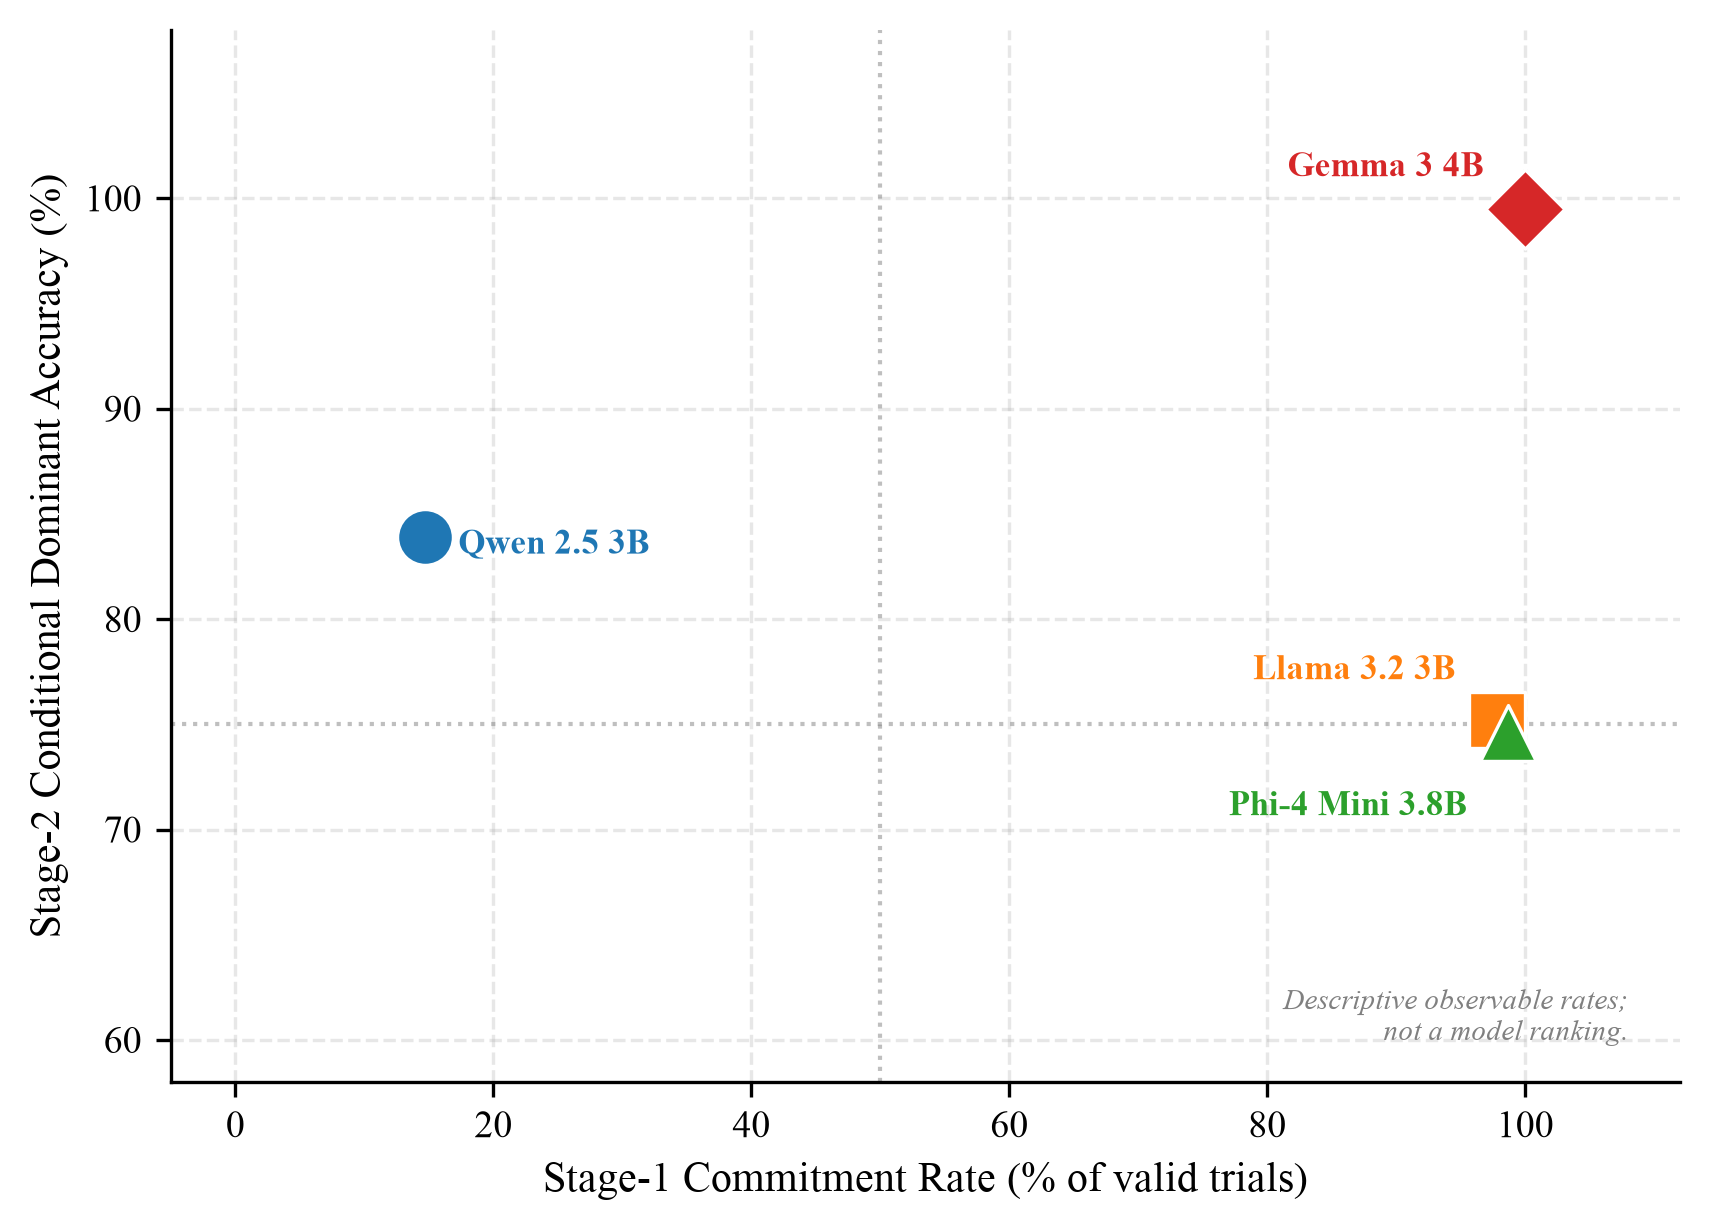
\includegraphics[width=0.78\linewidth]{figures/FigF_BehavioralProfile.png}
\caption{Two-Dimensional Behavioral Profile Based on Observable Rates. Scatter plot of empirical Stage-1 commitment rate (\% of valid trials) against Stage-2 conditional dominant accuracy (\% of committed non-parity trials). This descriptive visualization avoids separation-unstable regression coefficients.}
\label{fig:profile}
\end{figure}

By plotting observable commitment rates against conditional dominant-choice accuracy, the four models occupy distinct behavioral quadrants: Qwen combines selective commitment (14.7\%, 165/1,120) with high conditional accuracy (83.9\%, 135/161); Gemma exhibits universal commitment (100.0\%, 1,120/1,120) with near-ceiling conditional accuracy (99.5\%, 955/960); and Llama and Phi exhibit universal commitment (97.8\% [1,053/1,077] and 98.7\% [1,090/1,104]) with moderate conditional accuracy (75.2\% [679/903] and 74.6\% [701/940]).

\subsection{Threshold Follow-Up}
Across all 20 structural dilemmas in the $T=10$ control, the initial score satisfies $s_0 \ge 40 > T=10$, guaranteeing that the threshold was strictly satisfied prior to action selection. Full trial accounting shows that empirical commitment and conditional patterns persisted under this non-binding regime:
\begin{enumerate}
    \item \textbf{Qwen 2.5 3B:} Evaluated 1,120 valid trials (0 invalid), maintaining high non-directional abstention (84.0\%, 941 Indifferent) and committing on 179 trials; among the 176 non-parity committed trials, dominant-choice accuracy was 86.9\% (153/176), yielding a statistically significant payoff slope ($\hat\beta = 1.273$, $SE = 0.370$, $p = 5.8 \times 10^{-4}$, 95\% CI $[0.55, 2.00]$).
    \item \textbf{Llama 3.2 3B:} Evaluated 1,097 valid trials (23 invalid), committing on 1,078 trials (98.3\%, 19 Indifferent); on 925 non-parity committed trials, dominant accuracy was 74.1\% (685/925, $\hat\beta = 0.093$, $SE = 0.121$, $p = 0.443$, 95\% CI $[-0.14, 0.33]$).
    \item \textbf{Phi-4 Mini 3.8B:} Evaluated 1,107 valid trials (13 invalid), committing on 1,098 trials (99.2\%, 9 Indifferent); on 941 non-parity committed trials, dominant accuracy was 75.1\% (707/941, $\hat\beta = 0.101$, $SE = 0.123$, $p = 0.412$, 95\% CI $[-0.14, 0.34]$).
    \item \textbf{Gemma 3 4B:} Evaluated 1,120 valid trials (0 invalid), committing universally (100.0\%, 0 Indifferent); on 960 non-parity trials, Gemma selected the dominant option on 956 trials (99.6\%, 476/480 Option~A, 480/480 Option~B). Because Gemma achieved 100\% dominant accuracy across 800 of the 960 non-parity trials (making zero errors across all trials at ratios 1:2, 1:5, 1:9, 5:1, and 9:1) and committed only 4 errors (all occurring at the 2:1 ratio), the logistic likelihood encounters quasi-complete separation, driving the unpenalized MLE slope to an extreme value ($\hat\beta = 21.785, p=0.999$) with an uninformative asymptotic interval.
\end{enumerate}
These results verify that empirical payoff sensitivity in Qwen ($\hat\beta=1.273, p<0.001$) and ceiling directional accuracy in Gemma (99.6\%) persist independently of active threshold-crossing incentives. For Llama and Phi, however, payoff slopes under non-binding goals ($0.093$ and $0.101$) are not statistically distinguishable from zero ($95\%$ CIs $[-0.14, 0.33]$ and $[-0.14, 0.34]$); because their primary stabilized slopes were positive and bounded away from zero, threshold salience cannot be ruled out as a contributing factor for these two models. We also note that the follow-up models were estimated via dilemma-cluster-robust logistic regression, whereas primary Stage~2 specifications relied on dilemma cluster bootstraps and Firth penalization.

\subsection{Comparison with Forced-Choice Elicitation}
Figure~\ref{fig:forced_choice} compares observable choice behavior between the 3-option protocol and the matched 2-option forced-choice baseline across all 1,120 aligned trials for Qwen 2.5 3B.

\begin{figure}[!htbp]
\centering
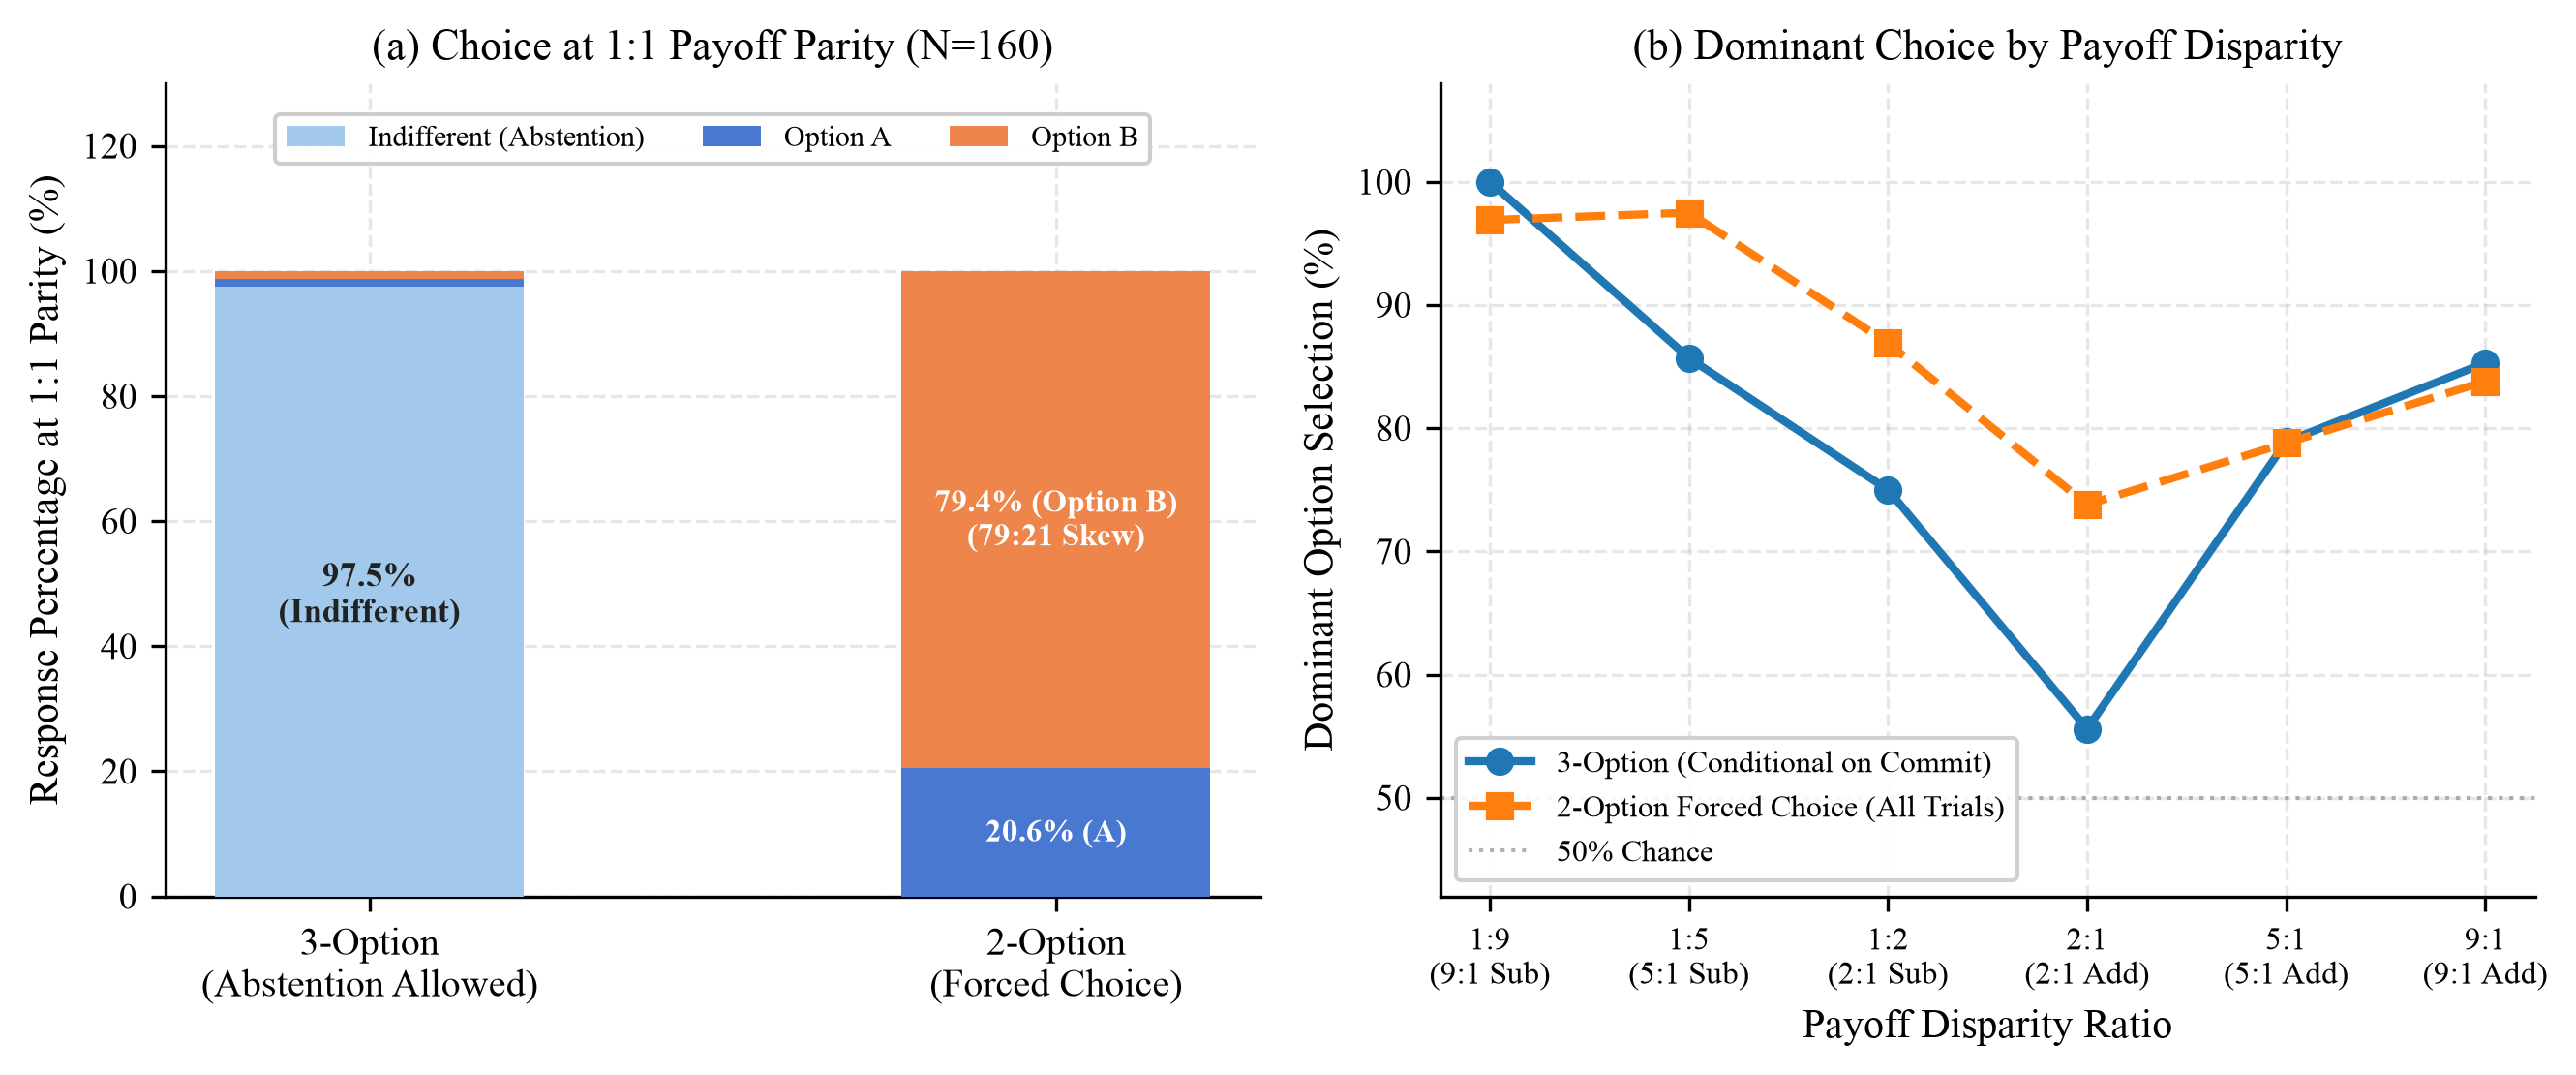
\includegraphics[width=0.78\linewidth]{figures/FigG_ForcedChoiceComparison.png}
\caption{Matched Comparison Between 3-Option Protocol and 2-Option Forced Choice (Qwen 2.5 3B, $N=1,120$). Panel~(a) shows that at 1:1 payoff parity, allowing abstention reveals 97.5\% indifference, whereas forced choice compels an asymmetric protocol-induced response (79.4\% Option~B). Panel~(b) compares dominant-choice accuracy across payoff disparity ratios.}
\label{fig:forced_choice}
\end{figure}

The empirical comparison yields two central findings:

First, at 1:1 payoff parity ($N=160$), where neither alternative is mathematically superior, the 3-option protocol revealed 97.5\% non-directional abstention (156/160 trials). In contrast, under forced choice, the protocol compelled a directional output, resulting in an asymmetric distribution: 79.4\% of choices selected Option~B (127/160; dilemma-cluster-aware 95\% CI $[74.6\%, 84.1\%]$, trial-level binomial 95\% CI $[72.4\%, 85.3\%]$) and 20.6\% selected Option~A (33/160) (Figure~\ref{fig:forced_choice}a). This pattern indicates that forced choice induces an asymmetric directional response at parity where the model would otherwise express indifference. Because Option~B occupied the second presentation position under standard labeling, this imbalance is consistent with either a second-position heuristic or a label bias toward Option~B.

To rigorously separate presentation position from action identity on all non-parity trials ($N=960$), we modeled dominant choice using the dominant-first indicator $\text{DominantFirst} \in \{+1, -1\}$ (defined as $+1$ when the mathematically dominant option is Option~A and $-1$ when Option~B) alongside payoff magnitude $|\log r|$, clustering standard errors at the structural dilemma level (20 clusters, applying the standard small-sample degrees-of-freedom adjustment $G/(G-1)$). The fitted logistic regression reveals both significant payoff sensitivity ($\hat\beta_{|\log r|} = 0.676$, $SE = 0.111$, $z = 6.08$, $p = 1.2 \times 10^{-9}$, 95\% CI $[0.458, 0.895]$) and a substantial negative effect of presenting the dominant alternative first ($\hat\beta_{\text{DominantFirst}} = -2.267$, $SE = 0.376$, $z = -6.04$, $p = 1.6 \times 10^{-9}$, 95\% CI $[-3.003, -1.531]$). In terms of observable accuracy across all 960 non-parity trials, when the dominant option was presented in the second slot (Option~B), Qwen selected it on 99.6\% of trials (478/480); when presented in the first slot (Option~A), accuracy fell to 72.9\% (350/480)---a 26.7 percentage-point position impairment (overall accuracy 86.25\%, 828/960). When adding an action identity indicator ($\text{DominantActionIsAdd} \in \{0, 1\}$), the position effect remains pronounced ($\hat\beta = -2.357$, $SE = 0.380$, $p = 5.5 \times 10^{-10}$), alongside a significant baseline preference for \textit{Subtract} ($\hat\beta = -1.695$, $SE = 0.200$, $p < 10^{-15}$). This action preference is consistent with a candidate action-label heuristic or semantic prior, though action label and Option~B/A slot cannot be fully disentangled without counterbalanced option naming. We emphasize that while controlling for action identity separates presentation order from operation type, it does not isolate a pure second-slot preference from a response-label preference for ``Option~B'', as slot and label remain aligned under standard presentation; we therefore interpret this as a joint label/position-associated response heuristic.

Second, examining the fate of the paired subset of trials where Qwen previously chose \textit{Indifferent} in the 3-option protocol (955 trials total; 799 on non-parity conditions) reveals that when forced to act, the model selected the mathematically dominant option on 86.5\% of these previously abstained trials (691/799). However, this paired subset is likewise heavily moderated by presentation slot: dominant-choice accuracy reaches 99.5\% (368/370) when the dominant option appears in Slot~2 (Option~B), but drops to 75.3\% (323/429) when it appears in Slot~1 (Option~A). This indicates that while Qwen retains latent numerical comparison capabilities rather than failing at basic arithmetic, forced choice does not elicit an unconfounded true preference, but rather interacts strongly with position heuristics. A compelling candidate explanation is a score-relative satisficing heuristic: because baseline scores are already progressing toward the threshold, the model treats both operations as acceptable when an indifference option is explicitly offered, but readily identifies the higher-payoff action when forced to decide. We emphasize, however, that satisficing remains a plausible hypothesis rather than a uniquely established causal mechanism, as prompt compliance, response formatting, and position heuristics also contribute. Forced choice conceals this behavioral complexity entirely, making an abstaining agent appear unconditionally directive while introducing severe position artifacts at parity.

\subsection{Ablations and Construct Validity Checks}
\label{sec:ablations_summary}

To directly evaluate alternative explanations regarding task incentives, presentation heuristics, action semantics, and decoding stability, we conducted five targeted control experiments and ablations, summarized in Table~\ref{tab:ablations_summary}.

\begin{table*}[!htbp]
\centering
\caption{Summary of Targeted Construct Validity Controls, Menu Ablations, and Robustness Checks.}
\label{tab:ablations_summary}
\footnotesize
\resizebox{\textwidth}{!}{%
\begin{tabular}{@{}lllcccp{5.5cm}@{}}
\toprule
\textbf{Control / Ablation} & \textbf{Targeted Construct} & \textbf{Evaluated Model ($N$)} & \textbf{Parity Abst.} & \textbf{Disparity Abst.} & \textbf{Commitment} & \textbf{Key Empirical Finding} \\
\midrule
Non-Zero Indifferent Payoff & Incentive structure & Qwen 2.5 3B ($N=280$) & 95.0\% (38/40) & 75.8\% (182/240) & 24.2\% & Non-zero payoff matching $\min(Q_A, Q_B)$ yields 95.0\% parity abstention, ruling out zero-payoff aversion as sole driver. \\
Menu-Slot Position Ablation & Recency vs.\ primacy & Qwen 2.5 3B ($N=72$) & --- & --- & 100.0\% & Placing \textit{Indifferent} in Slot~A extinguishes abstention (0.0\%), shifting choices to Slot~B (72.2\%) and Slot~C (27.8\%). \\
Lexical Label Variants & Semantic phrasing & Qwen 2.5 3B ($N=72$ ea.) & --- & --- & 2.8\%--23.6\% & Abstention persists across alternative tokens: 76.4\% for ``Neither'' and 97.2\% for ``No preference'' (vs.\ 31.9\% on matched 72 trials, 36.3\% across D01--D03). \\
Neutral Action/Slot Labels & Semantic bias \& slot tokens & Qwen 2.5 3B ($N=1,120$) & 65.6\% (105/160) & 12.4\% (119/960) & 87.6\% & Full $20\times 4\times 7\times 2$ factorial: abstract tokens surge disparity commitment from 16.8\% to 87.6\% (P3: 0.0\% to 96.2\%) with 98.7\% dominant accuracy and symmetric choices (50.9\%/49.1\%). \\
Stochastic Decoding & Sampling stability & Qwen 2.5 3B ($N=168$) & --- & --- & 16.7\% & Under $T=0.7$ across 3 seeds, abstention remains consistent (83.9\%, 83.9\%, 82.1\%; combined 83.3\% [77.0\%, 88.2\%]). \\
Second Domain Replication & Task framing generalizability & Qwen ($N=280$), Llama ($N=280$) & 100.0\% / 0.0\% & 98.3\% / 1.2\% & 1.4\% / 98.8\% & Resource scheduling replicates cross-model divergence; all 38 Llama invalids (13.6\%) resolved as directive under lenient parsing. \\
\bottomrule
\multicolumn{7}{p{\textwidth}}{\footnotesize Detailed experimental protocols, dilemma parameter specifications, prompt templates, and trial-level distributions for each control analysis are documented in Supplementary Sections~XI--XVI and Supplementary Tables~IX--XIII.}
\end{tabular}%
}
\end{table*}

\textit{Non-Zero Indifferent Payoff:} In the primary design, declining directional action yielded zero transformation points. To test whether Stage~1 measures directional commitment rather than aversion to a zero increment, we evaluated a matched condition where selecting \textit{Indifferent} awarded quality points matching the lower-payoff option: $Q_{\text{Indiff}} = \min(Q_A, Q_B)$ ($N=280$ trials on Qwen 2.5 3B across Dilemmas D01--D05; Supplementary Section~XIII). At 1:1 parity, where all three options offered identical positive rewards, Qwen continued to select \textit{Indifferent} on 95.0\% of trials (38/40, Wilson 95\% CI $[83.5\%, 98.6\%]$), identical to its zero-payoff baseline (38/40, 95.0\%). Under disparities, Qwen selected \textit{Indifferent} on 75.8\% of trials (182/240, Wilson 95\% CI $[70.0\%, 80.8\%]$) despite being strictly dominated by the higher-payoff action. This rules out zero-payoff aversion as the primary driver of abstention, indicating satisficing or prompt compliance.

\textit{Menu-Slot and Lexical Ablations:} Targeted menu variations on Qwen 2.5 3B ($N=72$ per condition across D01--D03; Supplementary Section~XIV) showed that while abstention is robust to alternative non-directional wording (76.4\% for ``Neither'' and 97.2\% for ``No preference''), placing the abstention option in the first menu slot (Option~A) completely extinguished abstention (0.0\%), shifting choices to Option~B (72.2\%) and Option~C (27.8\%). This indicates that abstention is mediated by menu recency and slot heuristics rather than an unconditional preference for inaction. In complementary stochastic evaluations at temperature $T=0.7$ across three independent random seeds ($N=168$; Supplementary Section~XV), abstention rates remained consistent across seeds (83.9\%, 83.9\%, 82.1\%; combined 83.3\%, Wilson 95\% CI $[77.0\%, 88.2\%]$), showing that high abstention is not a greedy decoding artifact ($T=0$).

\textit{Neutral-Label and Slot Counterbalancing:} In the primary stimulus design, actions were labeled ``Add'' and ``Subtract'' in menus labeled ``Option A'' and ``Option B''. To determine whether semantic connotations of the action labels (e.g., reluctance toward subtraction) or letter-based slot tokens contributed to Qwen's high abstention, we executed a full-factorial neutral-label experiment on Qwen 2.5 3B across all 20 structural dilemmas and all four phrasings ($N=1,120$ trials: $20\text{ dilemmas} \times 4\text{ phrasings} \times 7\text{ ratios} \times 2\text{ orders}$; Supplementary Section~XVI, Table~XIII). This experiment replaced ``Add'' and ``Subtract'' with abstract tokens (``Transformation Alpha'' and ``Transformation Beta'') and replaced options with numeric tokens (``Option 1'' and ``Option 2''). Under the full neutral factorial, Qwen chose \textit{Indifferent} on 65.6\% of parity trials (105/160). On disparity trials ($N=960$), Qwen committed directionally on 87.6\% of trials (841/960), achieving 98.7\% conditional dominant accuracy on committed choices (830/841). Disparity commitment surged across all four phrasings relative to the primary Add/Subtract baseline: P1 jumped from 15.8\% (38/240) to 95.4\% (229/240; 100\% dominant accuracy); P2 jumped from 41.7\% (100/240) to 100.0\% (240/240; 95.4\% dominant accuracy); P3 jumped from complete abstention (0.0\%, 0/240) to 96.2\% commitment (231/240; 100\% dominant accuracy); and P4 jumped from 9.6\% (23/240) to 58.8\% (141/240; 100\% dominant accuracy). Crucially, choices distributed near-symmetrically across action identities (428 Alpha [50.9\%] vs.\ 413 Beta [49.1\%]) and presentation slots (380 Option 1 [45.2\%] vs.\ 461 Option 2 [54.8\%]), in stark contrast to the primary baseline where choices were heavily skewed toward Subtract (60.9\%) and Option~B (84.5\%). These full-factorial results confirm and generalize our initial 70-trial pilot (which observed 85.0\% commitment across D01--D05 under P1): Qwen's headline ``abstention default'' is not an immutable model trait, but depends heavily on action-naming semantics and/or option tokens. Because this manipulation simultaneously altered both factors, isolating their independent marginal effects remains an open challenge.

\textit{Second Domain Replication (Resource Scheduling):} In a procedural holdout domain featuring server quota allocation dilemmas (Dilemmas H01--H05; Supplementary Section~XII), Qwen 2.5 3B and Llama 3.2 3B were evaluated across 280 balanced factorial trials each. For Qwen, all 280 trials were valid under strict parsing; Qwen chose \textit{Indifferent} on 98.6\% of trials (276/280; 100\% at parity, 98.3\% under disparities), committing on only 4 trials. For Llama, strict parsing classified 242 trials as valid and 38 trials as invalid (13.6\%, 38/280). Among strictly valid trials, Llama committed directionally on 98.8\% (239/242; 82.5\% dominant accuracy on committed non-parity trials, 165/200), choosing \textit{Indifferent} on only 1.2\% (3/242). Re-parsing the 38 invalid trials with a lenient parser that accepts comparative conversational commitments (e.g., \textit{``I will choose Option B, as it scores 9 quality points per entry...''}) resolved all 38 trials (17 Option~A, 21 Option~B; 0 Indifferent). Across the full 280-trial sample under lenient parsing, Llama committed directionally on 98.9\% of trials (277/280) with only 3 Indifferent choices (1.1\%), showing that the cross-model divergence in commitment replicates in the second domain regardless of parser strictness.

\section{Discussion}
\label{sec:discussion}

The core empirical finding is that forced-choice elicitation conflates two dissociable behavioral processes: the propensity to commit directionally and the sensitivity to payoffs conditional on commitment. When an explicit non-directional option is available, model behavior diverges sharply.

Qwen 2.5 exhibited an abstention-default profile, abstaining on 85.3\% of trials and committing primarily when payoff disparities were large. However, phrasing breakdowns reveal that this abstention was heavily language-dependent: under Phrasing~P3 (which referenced options being ``equivalent at your current score level''), Qwen abstained on 100\% of trials. This phrasing sensitivity is consistent with a candidate score-relative satisficing heuristic, though alternative explanations such as prompt compliance and template-specific lexical cues remain plausible. Indeed, an explicit wording ablation removing the score-level reference while retaining rule-equivalence framing preserved 100.0\% abstention (70/70 trials; Supplementary Section~XIV), indicating that the explicit score-level clause is not strictly necessary for universal abstention, though whether abstention is driven by broader rule-equivalence semantics or prompt compliance remains open.

Conversely, Llama, Phi, and Gemma exhibited directive defaults, committing on over 97\% of trials. For these models, forced-choice protocols would not distort commitment rates because the models rarely abstain. However, conditional on commitment, payoff sensitivity differed markedly: Gemma tracked payoffs accurately (conditional accuracy 99.5\%, Firth $\beta=1.531$), whereas Llama and Phi exhibited weaker sensitivity (Firth $\beta=0.282$ and $0.225$) and lower arithmetic comprehension on the C4 control (53.8\% and 71.0\%).

Crucially, presentation-position analysis reveals that the apparent conditional payoff sensitivity of Qwen and Phi under default framing is heavily undercut by position heuristics. For both architectures, dominant-choice accuracy plummets to chance levels (~49\%) whenever the mathematically dominant alternative appears in the disfavored slot (Option~A for Qwen [49.0\%], Option~B for Phi [49.3\%]), while reaching near-ceiling in the favored slot (100.0\% and 99.8\%, respectively). Furthermore, while Qwen achieved 100\% on C4 arithmetic comparisons, this isolated competence does not establish full comprehension of the interactive multi-turn task environment or threshold goal constraints. Thus, much of its fitted conditional sensitivity under default labeling represents an interaction with presentation heuristics rather than uncorrupted payoff valuation. Importantly, our neutral-label counterbalancing ablation reconciles this positional collapse: when action names and menu slots were counterbalanced with neutral tokens (Transformation Alpha/Beta, Option 1/2), choices split symmetrically across presentation slots (380 Option 1 [45.2\%] vs.\ 461 Option 2 [54.8\%]) and achieved 98.7\% dominant accuracy (830/841 committed trials) without slot bias. This shows that the severe position bias observed under default framing is not an immutable architectural limitation, but is elicited by the interaction between letter-based menu markers (Option~A/B) and action semantics. When combined with Llama's moderate first-slot bias (82.1\% vs.\ 68.4\%), Gemma 3 emerges as the sole evaluated architecture exhibiting genuine presentation-order invariance (99.0\% vs.\ 100.0\%).

Furthermore, when controlling for action identity in the 2AFC baseline, Qwen exhibits an independent baseline preference for \textit{Subtract} ($\hat\beta = -1.695, p < 10^{-15}$). This indicates that operation names may carry latent semantic priors: despite identical positive reward structures, the connotations of reduction or pruning vs.\ addition introduce subtle linguistic biases, though action label and Option~B/A slot cannot be fully disentangled without counterbalanced option naming. This reinforces that model choices in procedural pipelines reflect a complex interaction of numerical payoffs, presentation slots, and action labeling.

Finally, our findings present an informative contrast with recent evaluations in open-ended domains: while Mahajan et al.~\cite{mind_the_gap_2026} observed Gemma 3 4B choosing ``Equal Preference'' in ~70\% of conversational risk dilemmas, the same model in our quantitative data-pipeline environment exhibited a strictly directive default (0.0\% abstention). This shows that default commitment is not a static property of model weights, but is co-determined by the task framing and elicitation architecture.

\section{Limitations and Threats to Validity}
\label{sec:limitations}

Several important limitations must be emphasized.

First, the evaluation is restricted to four locally deployed models in the 3--4B parameter tier under 4-bit medium quantization (\texttt{Q4\_K\_M}). While evaluating this tier enables exhaustive factorial testing across 4,480 trials and matched controls, it does not establish generality across larger open-weight models (e.g., 70B parameter models) or frontier proprietary systems. Local deployment of unquantized 16-bit floating-point (FP16) builds was constrained by local single-machine hardware boundaries (8.0~GB unified system RAM, 5.30~GiB Metal allocatable ceiling, and 5.20~GiB available storage; see Supplementary Section~XI, Table~VIII), as FP16 checkpoints require 6.4--8.0~GB for weights alone plus runtime context buffers, which is expected to exceed allocatable Metal memory limits or available disk space. To facilitate unquantized evaluation, we provide a self-contained cloud execution pipeline and interactive notebook (Supplementary Section~XVII) designed for free Google Colab or Kaggle T4 GPU instances (16~GB VRAM) supporting unquantized FP16 checkpoints and larger 7B/8B models. Evaluating FP16 builds across the full 4,480-trial design remains an open objective for future work.

Second, while the procedural task environment encompasses 20 structural dilemmas and replicates in a resource scheduling domain (Dilemmas H01--H05), both domains feature quantitative quality payoffs. Expanding evaluation to non-numeric decision tasks, unstructured multi-agent games, and broader conversational reasoning environments is necessary to determine the generalizability of the observed hurdle decomposition.

Third, our counterbalancing ablations show that commitment is sensitive to prompt framing and tokenization: across a full 1,120-trial factorial design, Qwen's disparity commitment surged from 16.8\% to 87.6\% (and from 0.0\% to 96.2\% under phrasing P3) when actions and slot tokens were simultaneously neutralized, while moving the abstention option to Slot~A completely extinguished abstention. These results indicate that commitment propensity in smaller models is not an invariant behavioral constant, but interacts with presentation recency, letter-vs-number option markers, and action semantics. Disentangling the individual causal contributions of action names versus slot tokens via independent full-factorial counterbalancing across all models remains an open empirical challenge.

Fourth, while we evaluated a matched 2AFC baseline on Qwen 2.5 3B (showing that forced choice induces a 79:21 response imbalance at parity and introduces severe position sensitivity, $\hat\beta_{\text{DominantFirst}} = -2.267$, $p < 10^{-8}$ under cluster-robust inference), extending matched forced-choice baselines across all evaluated model families and larger open-weight architectures remains an important objective for future benchmarking. For Llama 3.2, Phi-4 Mini, and Gemma 3, primary 3-option behavior is already functionally forced-choice (>97.8\%--100\% directional commitment), making Qwen uniquely informative for isolating the distortions introduced when abstention is omitted.

Fifth, 43 Llama trials (3.8\%) and 16 Phi trials (1.4\%) in the primary domain returned invalid responses that failed to match permitted output strings under strict parsing, concentrated under Phrasing~P4 where models generated conversational explanations. Bounding sensitivity analysis shows that Stage~2 conditional dominant accuracy is robust to these exclusions: incorporating leniently parsed conversational commitments yields Stage~2 conditional dominant accuracy of 75.69\% for Llama (713/942, vs.\ 75.19\% strict; $\Delta = +0.50\%$) and 74.92\% for Phi (714/953, vs.\ 74.57\% strict; $\Delta = +0.35\%$), showing that parser strictness does not affect substantive findings.

Sixth, the conditional Stage~2 analysis exhibits quasi-complete separation for highly sensitive models. While Firth penalized regression guarantees finite estimates and bounded profile intervals, standard asymptotic inference remains approximate.

Seventh, the operational \textit{Indifferent} category is intentionally agnostic about internal causes. Abstention may reflect genuine indifference, ambiguity, safety caution, or prompt heuristics; categorical outputs alone cannot identify latent cognitive states.

Finally, reported $p$-values are nominal without multiplicity adjustment. Structural dilemma clustering was addressed via 10,000-resample blocked bootstraps for Stage~2 conditional specifications, alongside dilemma-cluster-robust sandwich variance estimation for Stage~1 hurdle and 2AFC models.

\section{Conclusion}
\label{sec:conclusion}

Across four instruction-tuned small model families (3--4B parameters), decomposing preference elicitation into directional commitment and conditional direction revealed distinct behavioral profiles that single-turn forced-choice protocols obscure. Models varied from heavily abstaining to universally directive under default framing, though targeted counterbalancing shows that commitment propensity is sensitive to action semantics and prompt formatting. Furthermore, conditional payoff sensitivity co-varied with numerical comprehension and presentation position, alongside candidate action-label heuristics. These findings indicate that observed preferences in smaller models can be sensitive to protocol-induced artifacts and motivate the adoption of abstention-aware, position-controlled evaluation frameworks.

\section*{Data and Code Availability}
All prompt templates (verbatim, Table~\ref{tab:phrasings_full}), structural dilemma specifications, and example turn-by-turn transcripts are included in this paper and in the supplementary material (Supplementary Sections~I--XVIII). All experimental code, prompt templates, structural dilemma specifications (\texttt{m3v2\_stimuli.json}), deterministic response parsers, analysis scripts, and raw trial data are permanently available in an open-access repository at \url{https://github.com/CodeShrek/LLM-Preference-Diagnostics}.

\bibliographystyle{IEEEtran}
\bibliography{references}

\end{document}
